\documentclass[12pt]{report}


% Zařadit literaturu do obsahu
\usepackage[nottoc,notlot,notlof]{tocbibind}

% Umožňuje vkládání obrázků
\usepackage[pdftex]{graphicx}

% Odkazy v PDF jsou aktivní; navíc se automaticky vkládá
% balíček 'url', který umožňuje např. dělení slov
% uvnitř URL
\usepackage[pdftex]{hyperref}
\hypersetup{colorlinks=true,
  unicode=true,
  linkcolor=black,
  citecolor=black,
  urlcolor=black,
  bookmarksopen=true}

% Při používání citačního stylu csplainnatkiv
% (odvozen z csplainnat, http://repo.or.cz/w/csplainnat.git)
% lze snadno modifikovat vzhled citací v textu
\usepackage[numbers,sort&compress]{natbib}


% me package
\usepackage{float}
%\usepackage{subfig}
\usepackage{siunitx}
\usepackage[czech]{babel}
\usepackage{tabularx}
\usepackage{caption}
\usepackage{subcaption}
\usepackage{pdfpages}

%%%%%%%%%%%%%%%%%%%%%%%%%%%%%%%%%%%%%%%%%%%%%%%%%%%%%%%%%%
%
% VLASTNÍ TEXT PRÁCE
%
%%%%%%%%%%%%%%%%%%%%%%%%%%%%%%%%%%%%%%%%%%%%%%%%%%%%%%%%%%

\makeatletter
\def\@makechapterhead#1{%
  {\parindent \z@ \raggedright \normalfont
    \Huge\bfseries
    \ifnum \c@secnumdepth >\m@ne
        \hangindent=1.5em
        \noindent\hbox to 1.5em{\thechapter\hfil}%
    \fi%
    #1\par\nobreak
    \vskip 40\p@
  }}
\def\@makeschapterhead#1{%
  {\parindent \z@ \raggedright \normalfont
    \interlinepenalty\@m
    \huge \bfseries  #1\par\nobreak
    \vskip 40\p@
  }}
\makeatother


\begin{document}
%

\begin{titlepage}
\centerline{
\includegraphics[width=10cm]{img/logo.jpg}}
\begin{center}
\vspace{30px}
{\huge
\textbf{Úvod do uživatelských rozhraní}\\
\textbf{KIV/UUR}\\
\vspace{1cm}
}
{
\vspace{1cm}
}
\vspace{1cm}
{\large
Pavel Třeštík\\
}
{\normalsize
A17B0380P
}
\end{center}
\vspace{\fill}
\hfill
\begin{minipage}[t]{7cm}
\flushright
\today
\end{minipage}
\end{titlepage}
%
%
%
%\maketitle
\tableofcontents
%
%
%
\chapter{Zadání}
Výsledkem práce má být mobilní aplikace na platformě Android. Aplikace má sloužit
ke správě skladu medu. V aplikaci je nutné mít přehled o produktech. Produkty mají
různé informace, které jsou o nich ukládány a měly by v aplikaci být zjistitelné.
Mezi tyto informace patří samozřejmě počet uskladněných produktů, který je třeba měnit.

Aplikace dále umožní zadávat objednávky. Zadáním objednávky se sníží počet produktů.
Objednávky by mělo být možné prohlížet a určit, které objednávky jsou stále aktivní (nesplněné)
a které objednávky již byly dokončeny.
%
\section{Návrh realizace zadání}
V rámci aplikace je tedy třeba udělat jak "back-end", tak "front-end". 

Back-end manipuluje s daty. Data musí být perzistentní, tudíž je nutné je ukládat.
Možností ukládání je několik. Lze ukládat například do souboru s vlastní strukturou, použít
některý ze známých a využívaných formátů jako XML, JSON nebo použít databázi. Čím déle by 
aplikace byla používána bez mazání dat, tak by při zvolení např. XML narůstala režie a soubor by 
zabíral více místa.
Protože již existuje e-shop, je tady možnost, že by se v budoucnu aplikace mohla provázat s e-shopem, ale
to nebyl ani sekundární objektiv této práce. Ale vzhledem k této možnosti, je pravděpodobně nejlepším
řešením použít databázi. Dobře navržená databáze by neměla mít velkou režii jako například XML. A dále
by nemělo být složité udělat databázi, která je sdílena mezi aplikací a e-shopem pro možnou budoucí
integraci.

Front-end je pouze grafické rozhraní, skrz které uživatel manipuluje data. Z aplikace je třeba zjistit
stavy produktů. Zadávat i mazat produkty. Dále zadávat objednávky a prohlížet je.
%
\chapter{Implementace}
Aplikace je psána pro Android v jazyce Java. Minimální cílová API úroveň je 21, což odpovídá Android
verzi 5.0 "Lollipop". Pro back-end je použita databáze SQLite, ke které API poskytuje přístup.
\section{Struktura projektu}
Projekt má adresářovou strukturu znázorněnou na Obrázku \ref{img:project_struct}. Tato struktura
je vygenerována Android Studiem, ve kterém jsem projekt vytvářel a myslím si, že je docela přehledná a proto
nebylo třeba ji měnit. Navíc měnit tuto strukturu je obtížné, protože by bylo třeba manuálně upravit build 
skripty.

Ačkoliv to pravděpodobně není očividné z adresářové struktury, tak projekt dodržuje 3 vrstvou architekturu.
S databází pracují některé třídy v balíku \texttt{model}. Funkce těchto tříd jsou poté užívány kontrolery
v balíku \texttt{controllers}. Kontrolery buď předávají data modelu do GUI nebo opačným směrem.

\begin{figure}[H]
        \centering
        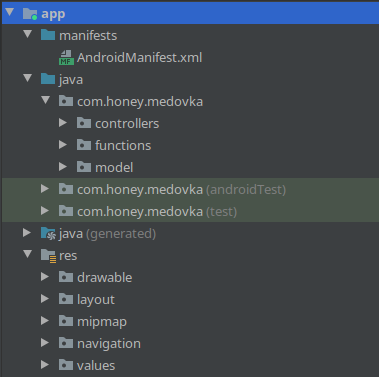
\includegraphics[width=0.5\textwidth]{img/dir_structure.png}
        \caption{Struktura projektu}
        \label{img:project_struct}
\end{figure}
%
\section{Použité GUI prvky}
\subsection{Elementární prvky}
Pro navigaci aplikací jsou použité tlačítka (Button). V jedné tabulce je použito obrázkové tlačítko
(ImageButton), které má obrázek "+" a slouží k přidání řádky do tabulky. Dále jsou používány 
TextView pro popisky.Pro zadání jak číselných tak slovních hodnot je použit EditText, který umožňuje
zvolit zadávaný typ a nedovolí uživateli zadávat např. písmena do číselného vstupu. Dalším způsobem
zadávání jsou výběrové seznamy (Spinner).
\subsection{Pokročilé prvky}
\subsubsection{RecyclerView}\label{rv}
Je to posuvný seznam, který zobrazuje objekty na který je typovaný.
Tento prvek má v podstatě nahrazovat TableLayout a má být efektivnější zejména pro velký počet prvků.
K jeho použití je třeba implementovat vlastní Adapter, což je třída, která uchovává a spravuje prvky listu
a také zařizuje jejich zobrazení. K jejich zobrazení Adapter vnitřně rozšiřuje třídu ViewHolder, která 
převádí objekt na GUI elementy, které definují, jak objekt v seznamu vypadá.
\subsubsection{TableLayout}
Podobně jako RecyclerView umožňuje zobrazit položky v řádkách pod sebou. Programátor musí stejně jako u
RecyclerView definovat jak řádka vypadá, ale řádka není vázaná k určitému objektu a tudíž je v tabulce
snadné mít řádky různých typů. Nevýhodou je, že tabulky nejsou nativně posuvné a proto musí být navíc obaleny
ScrollView prvkem. Tabulky je lepší využívat pro statický obsah, ovšem je možné řádky dynamicky přidávat
a ubírat.
%
\section{Datový model}
Jak již bylo zmíněno základem aplikace je databáze. Jedná se o SQLite databázi.
Na obrázku \ref{fig:model} je relační diagram databáze, který aplikace momentálně používá.
Aplikace má sloužit ke správě produktů a umožnit zadávat objednávky. Model zahrnuje všechny důležité
vlastnosti důležitých tabulek (produktů a objednávek). Ovšem i přes to by se mohly najít vlastnosti 
těchto objektů, které by se do modelu mohly přidat. Největší změnou, co by se mě osobně na modelu líbila,
by bylo udělat vazby mezi atributy, protože atributy jsou na sobě často závislé, ale v rámci této
práce jsem musel model zjednodušit z časových důvodů.

\begin{figure}[H]
	\centering
	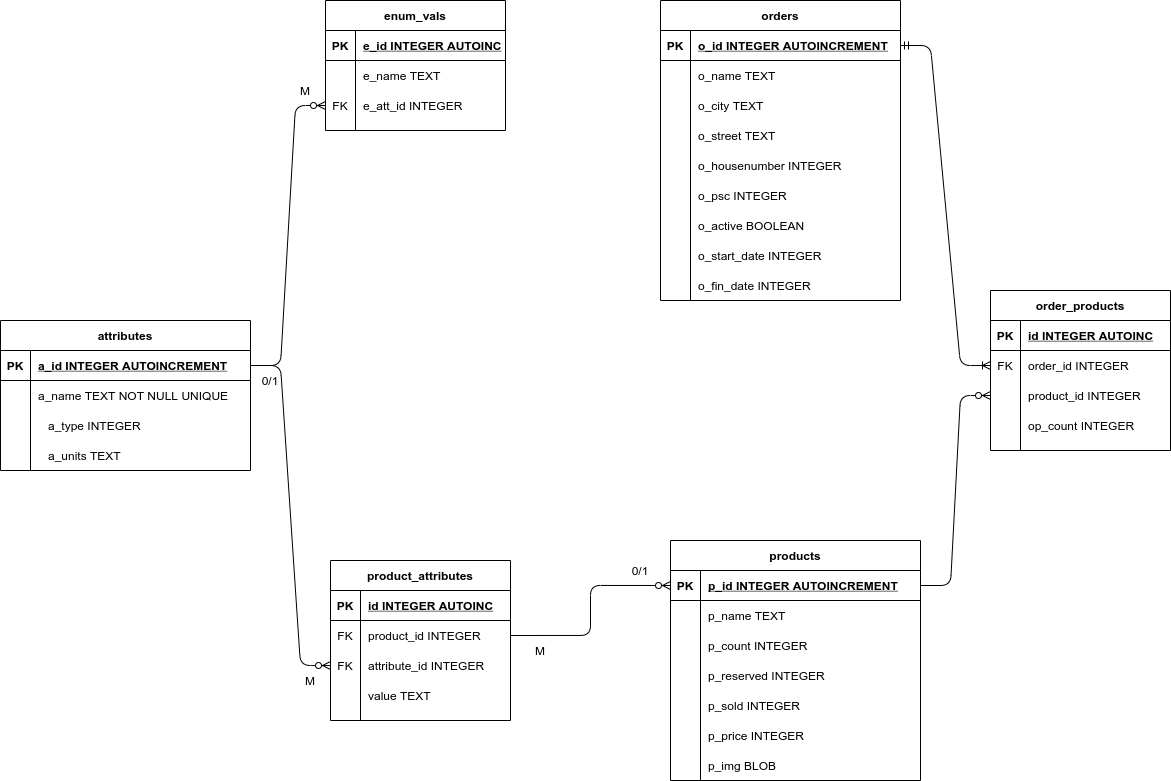
\includegraphics[width=1.13\textwidth,angle=270,origin=c]{img/medovka_diagram.png}
	\caption{Model databáze}
	\label{fig:model}
\end{figure}
%
\chapter{Rozložení GUI}
%
\section{Menu}
%
\begin{figure}[H]
	\centering
	\begin{subfigure}{.3\textwidth}
	  \centering
	  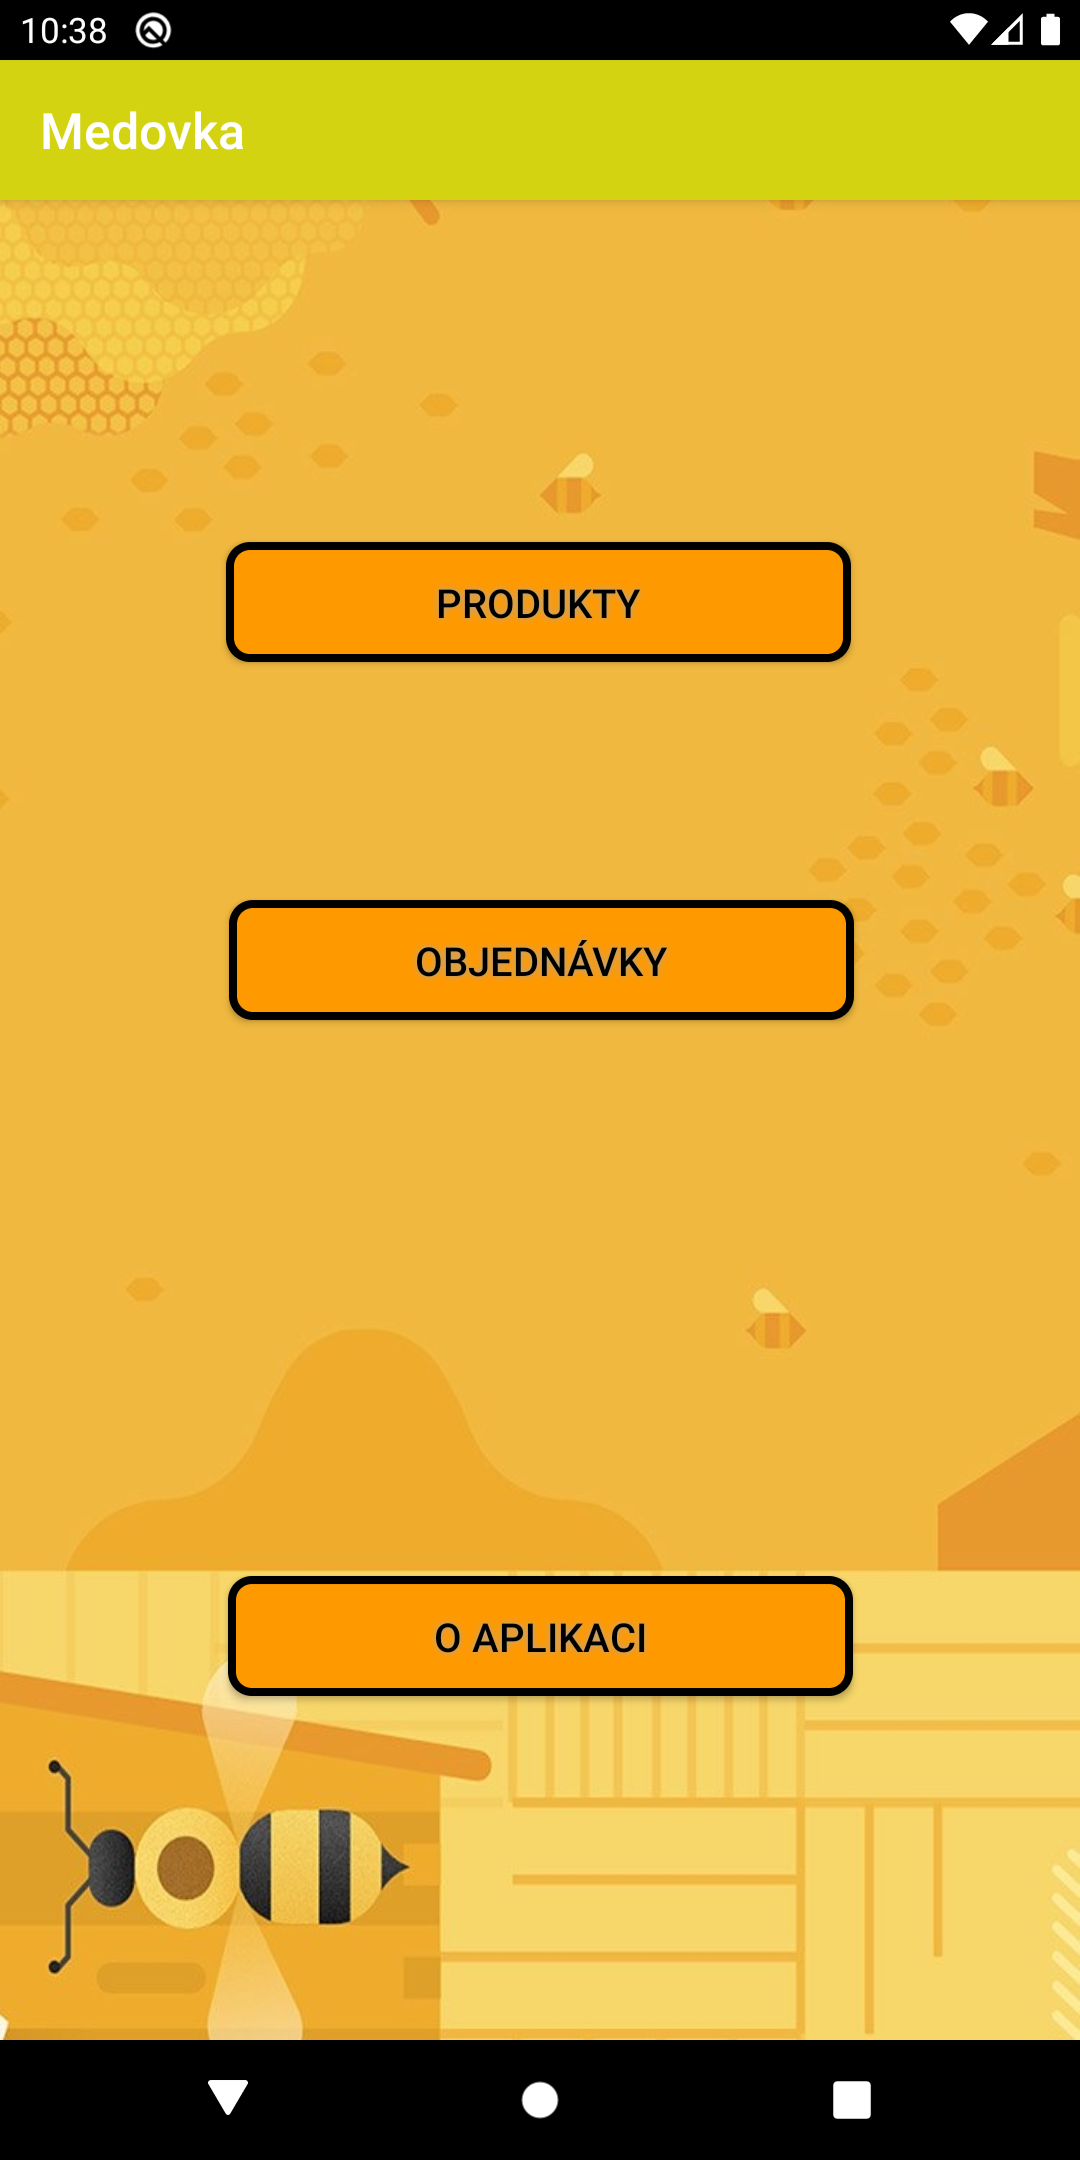
\includegraphics[width=\textwidth]{img/main_window.png}
	  \caption{Hlavní menu}
	  \label{fig:main_menu_img}
	\end{subfigure}
	%
	\begin{subfigure}{.3\textwidth}
	  \centering
	  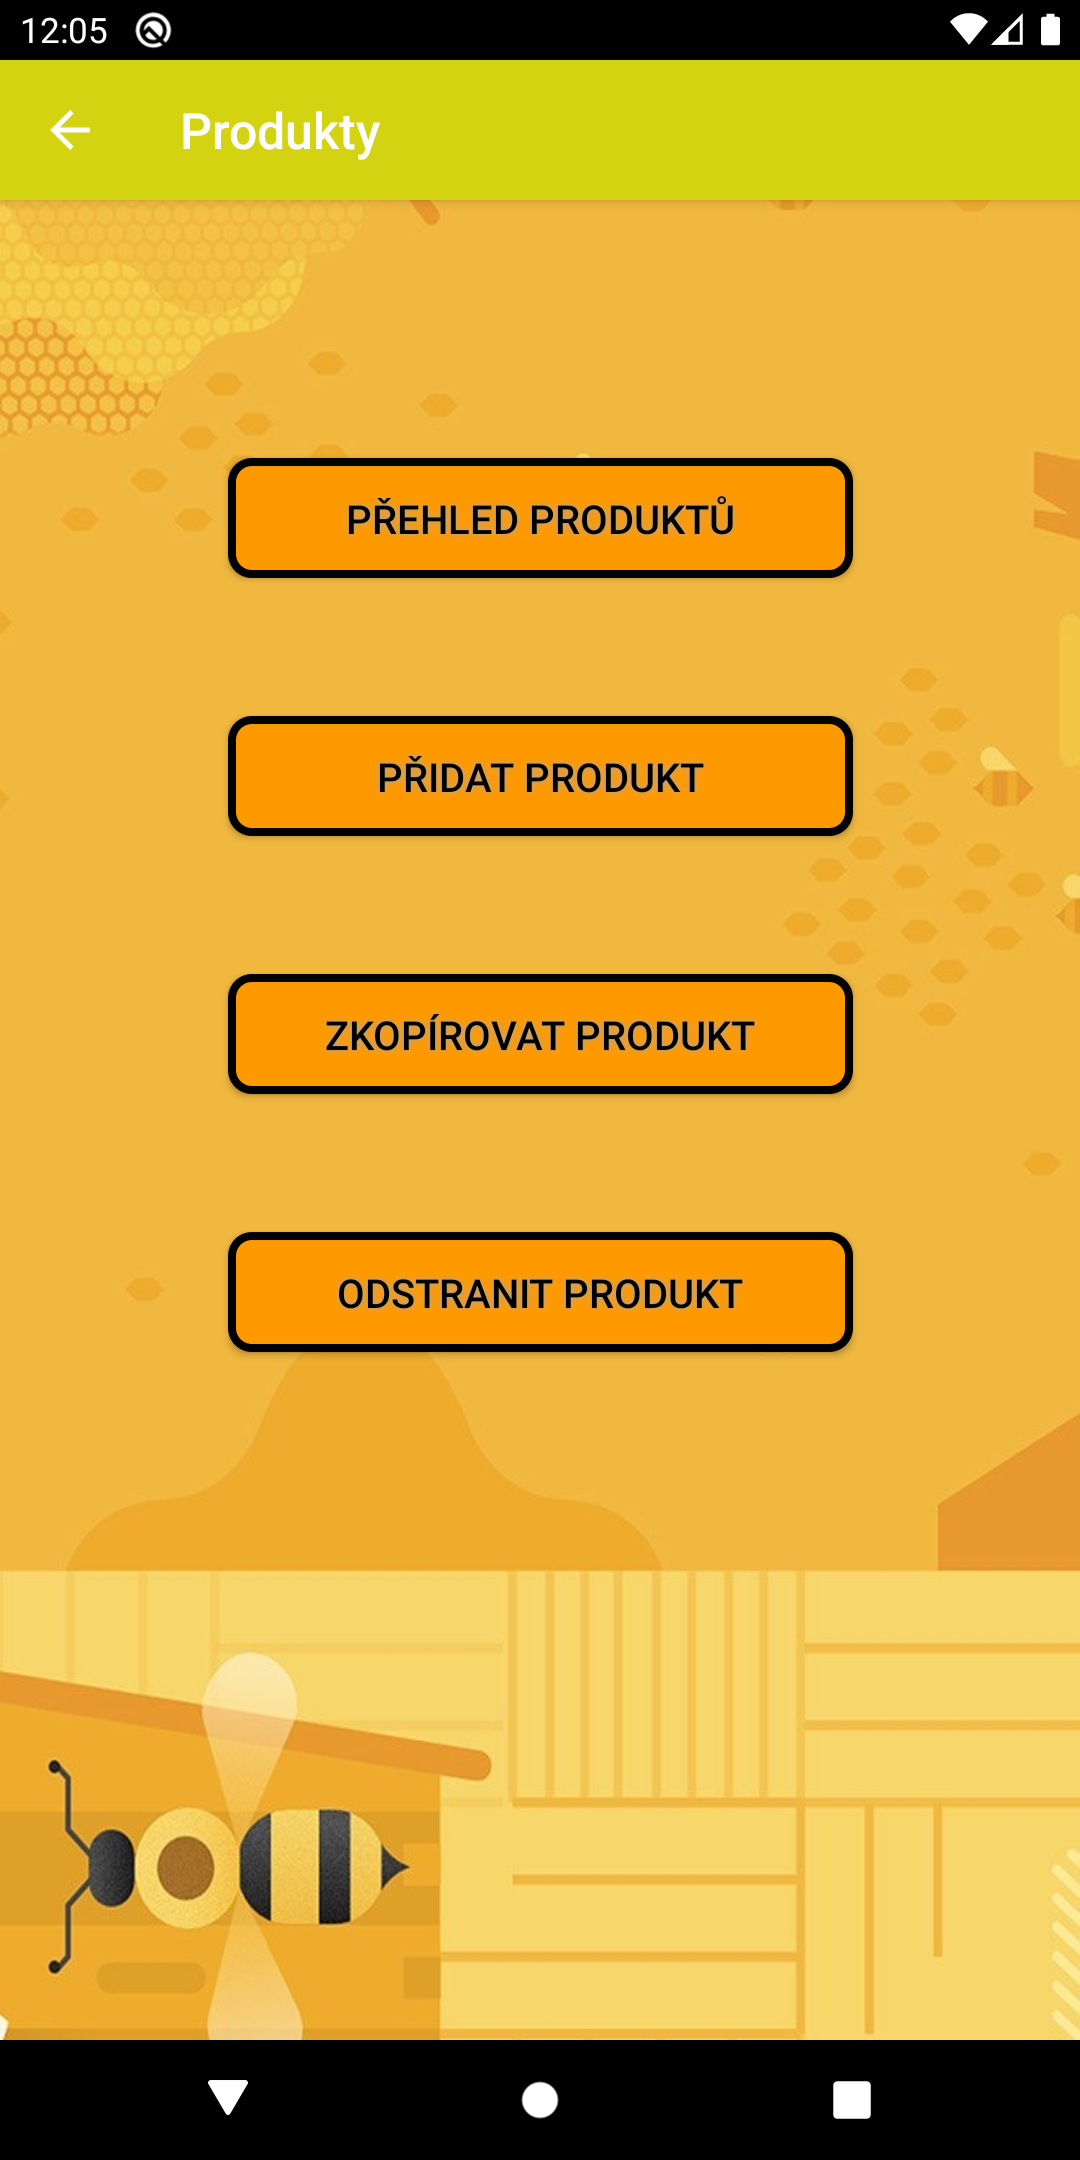
\includegraphics[width=\textwidth]{img/product_menu.png}
	  \caption{Menu produktů}
	  \label{fig:product_menu_img}
	\end{subfigure}
	%
	\begin{subfigure}{.3\textwidth}
	  \centering
	  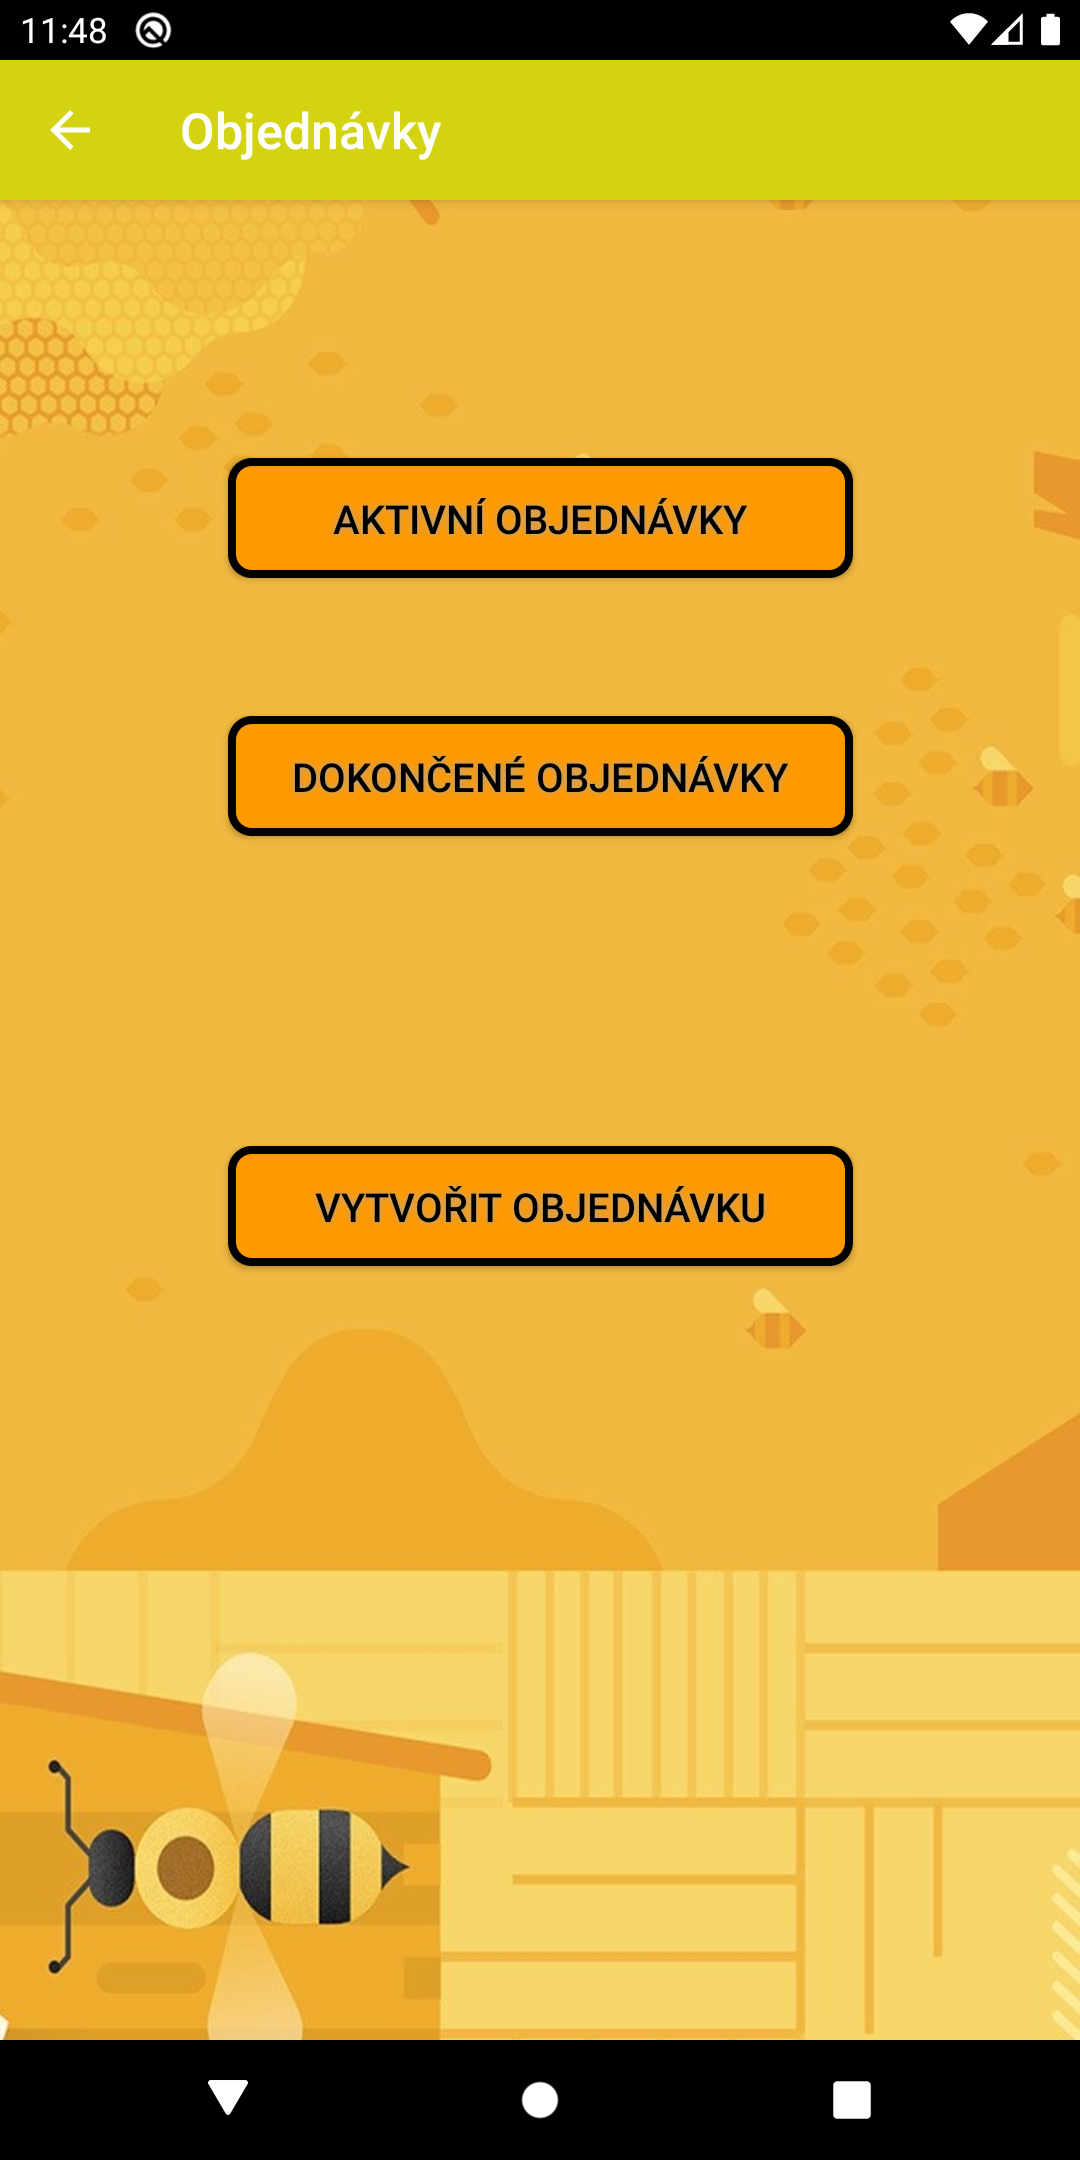
\includegraphics[width=\textwidth]{img/order_menu.png}
	  \caption{Menu objednávek}
	  \label{fig:order_menu_img}
	\end{subfigure}
	%
	\caption{Menu aplikace}
	\label{fig:menus_cont}
\end{figure}
%
Ve skupině obrázků \ref{fig:menus_cont} jsou menu, která aplikace obsahuje. Menu obsahuje pouze tlačítka,
které slouží k navigaci na jinou obrazovku. V obrázku \ref{fig:main_menu_img} tlačítko \texttt{Produkty}
vede na menu produktů (obrázek \ref{fig:product_menu_img}) a tlačítko \texttt{Objednávky} vede na menu 
objednávek (obrázek \ref{fig:order_menu_img}).
%
\section{Seznamy}
\begin{figure}[H]
	\centering
	\begin{subfigure}{.45\textwidth}
	  \centering
	  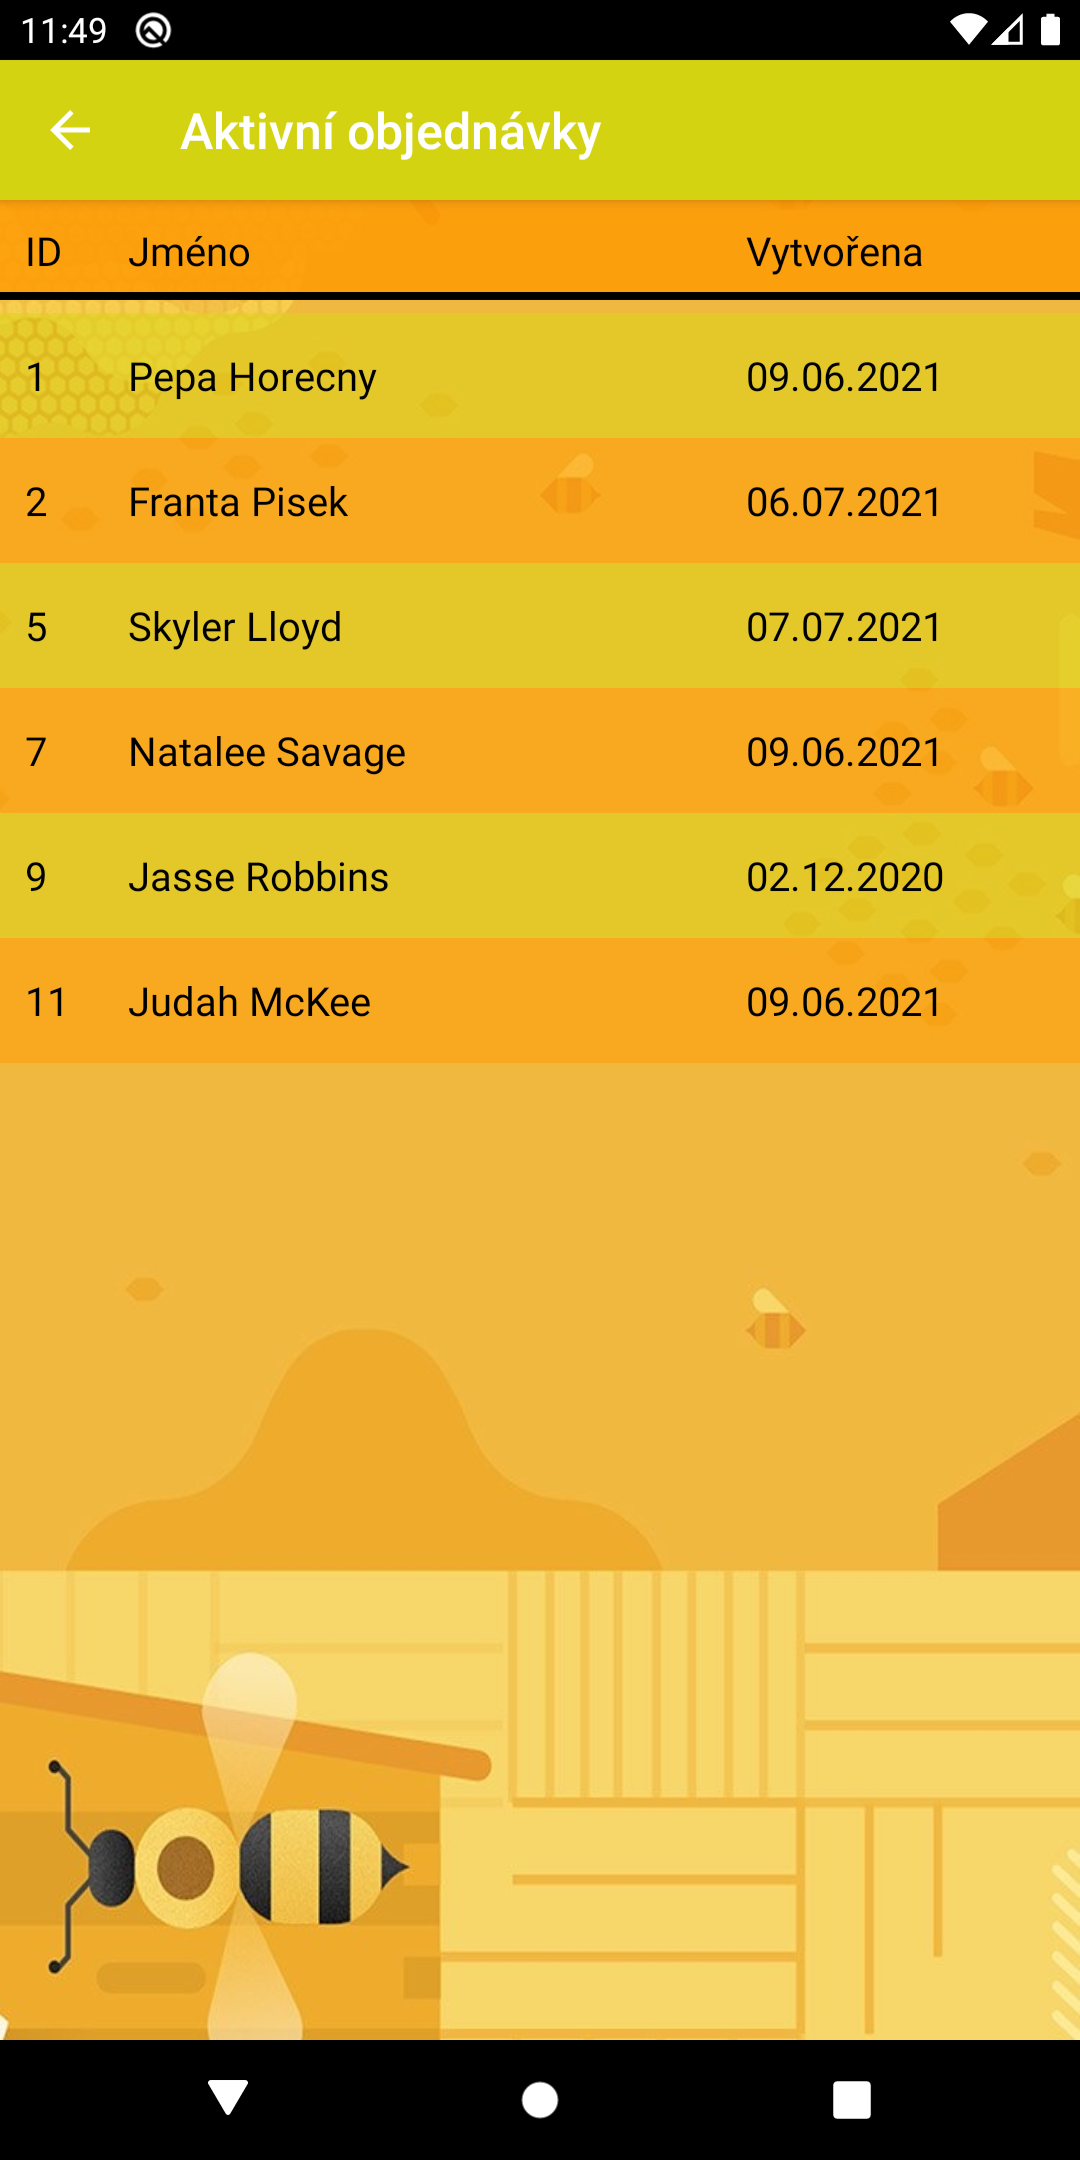
\includegraphics[width=\textwidth]{img/order_list.png}
	  \caption{Seznam objednávek}
	  \label{fig:order_list_img}
	\end{subfigure}
	%
	\begin{subfigure}{.45\textwidth}
	  \centering
	  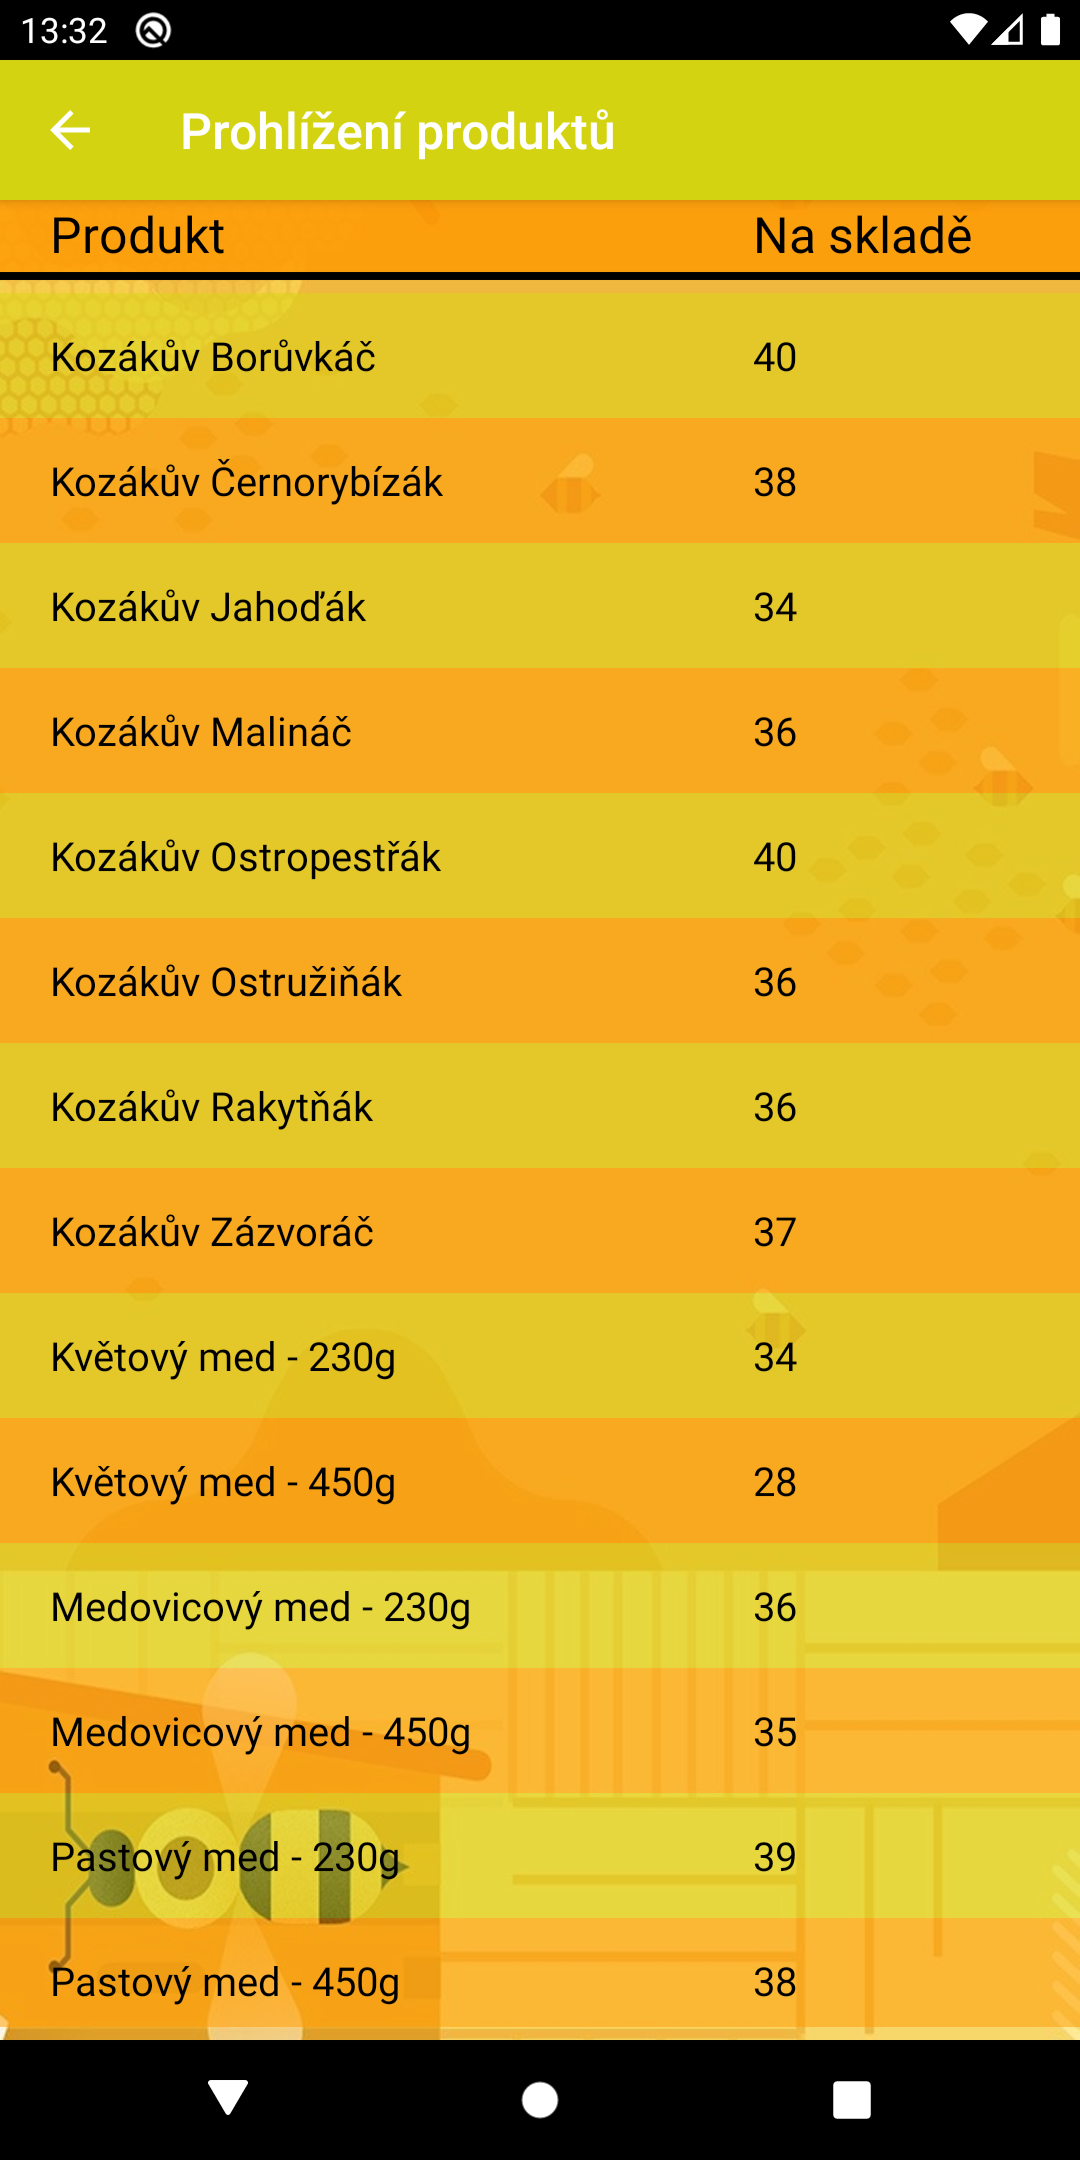
\includegraphics[width=\textwidth]{img/product_list.png}
	  \caption{Seznam produktů}
	  \label{fig:product_list_img}
	\end{subfigure}
	%
	\caption{Příklady seznamů}
	\label{fig:list_cont}
\end{figure}
%
Ve skupině obrázků \ref{fig:list_cont} jsou příklady dvou seznamů (RecyclerView, popsán v \ref{rv}).

Seznam použit na obrázku \ref{fig:order_list_img} je použit pro zobrazení aktivních i dokončených objednávek
(viz menu \ref{fig:order_menu_img}).

Seznam použit na obrázku \ref{fig:product_list_img} je použit pro zobrazení přehledu produktů, vybrání
produktu ke kopírování a odstranění produktu (viz menu \ref{fig:product_menu_img}).
Ačkoliv je použit stejný fragment, položky v každém seznamu 
vypadají trochu jinak. V přehledu je u položky počet produktů na skladě. U odstranění
produktů je místo počtu položek checkbox pro označení vybraných produktů. V seznamu
pro kopírování je pouze jméno produktu.
%
\section{Zobrazení detailů}
\begin{figure}[H]
	\centering
	\begin{subfigure}{.45\textwidth}
	  \centering
	  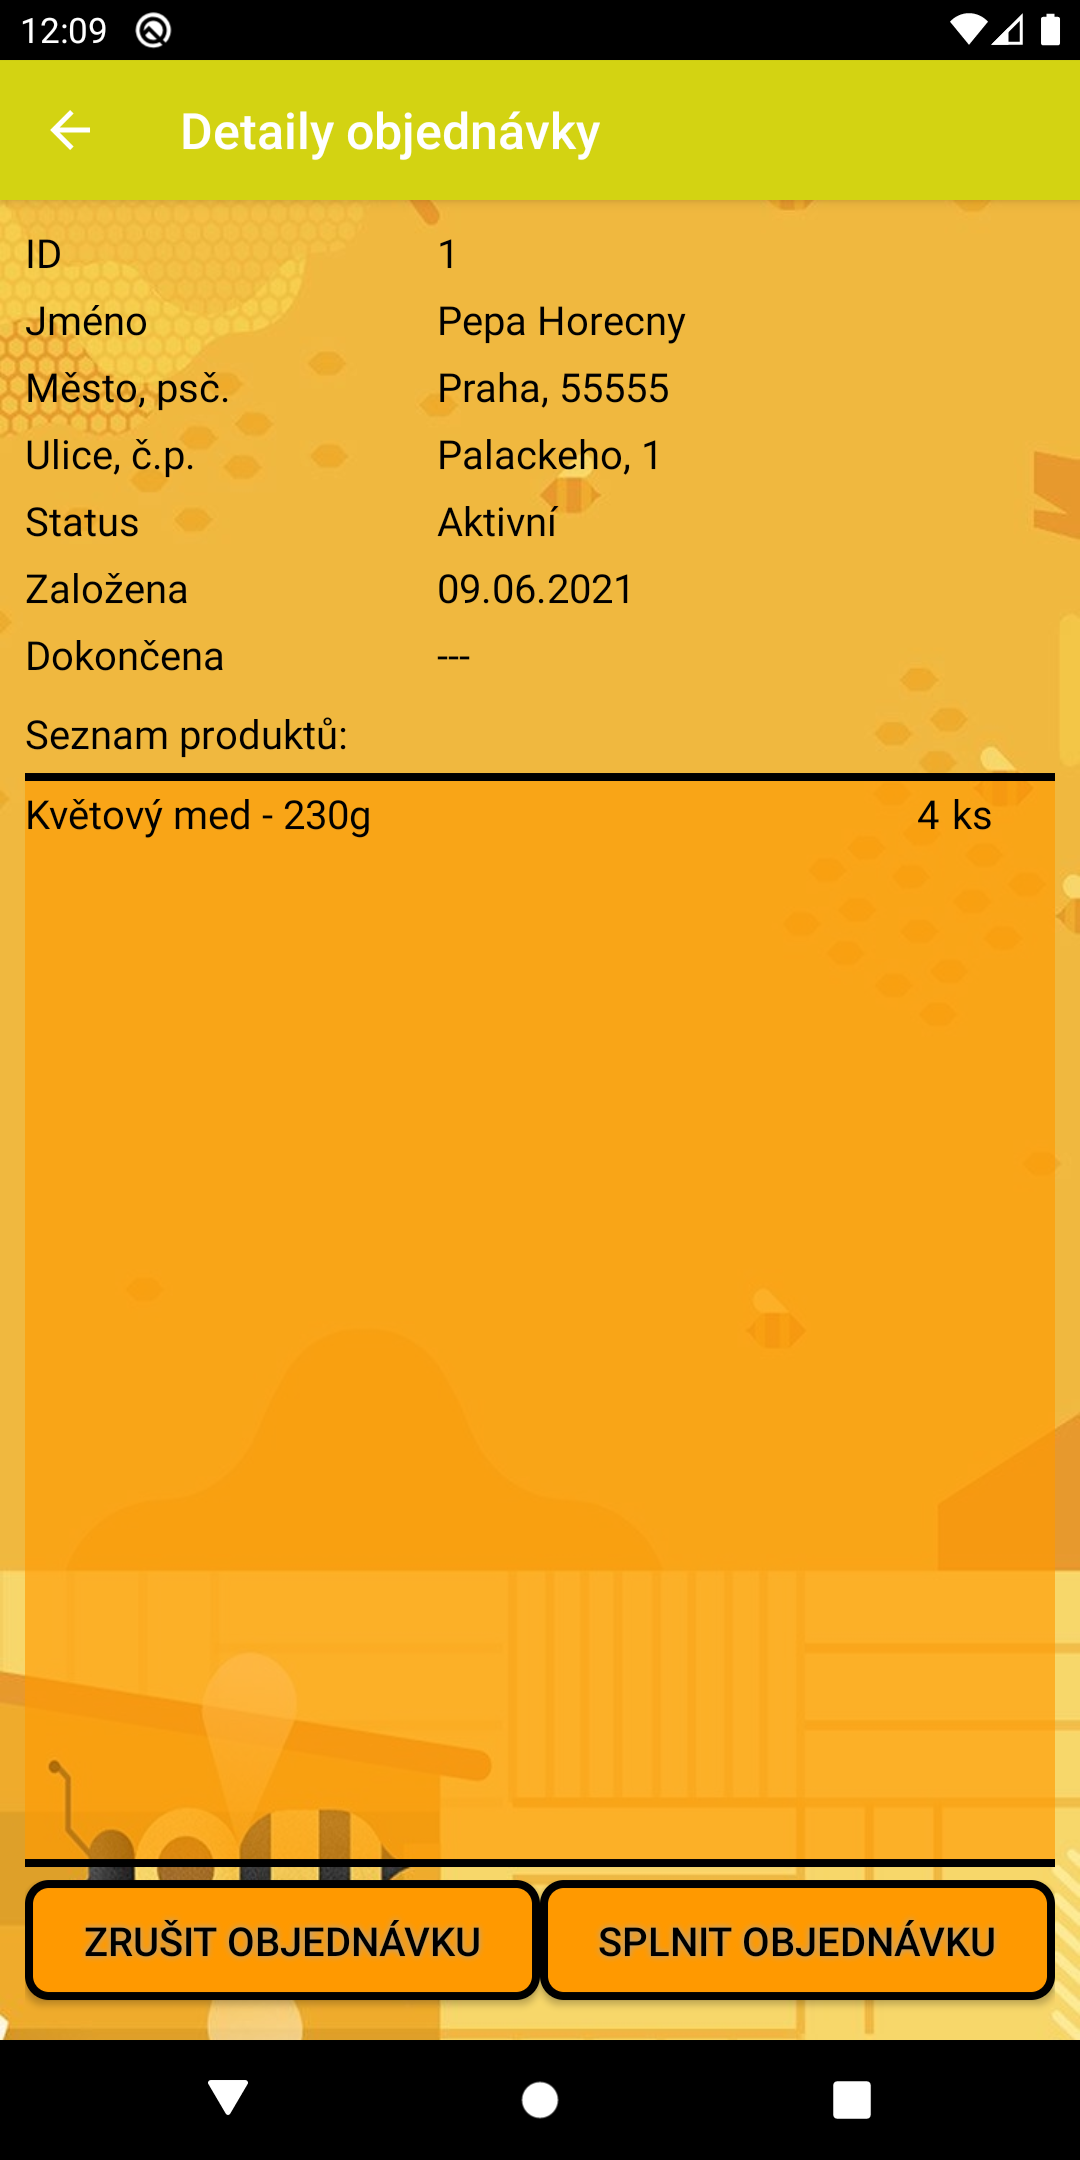
\includegraphics[width=\textwidth]{img/order_detail.png}
	  \caption{Detail objednávky}
	  \label{fig:order_det}
	\end{subfigure}
	%
	\begin{subfigure}{.45\textwidth}
	  \centering
	  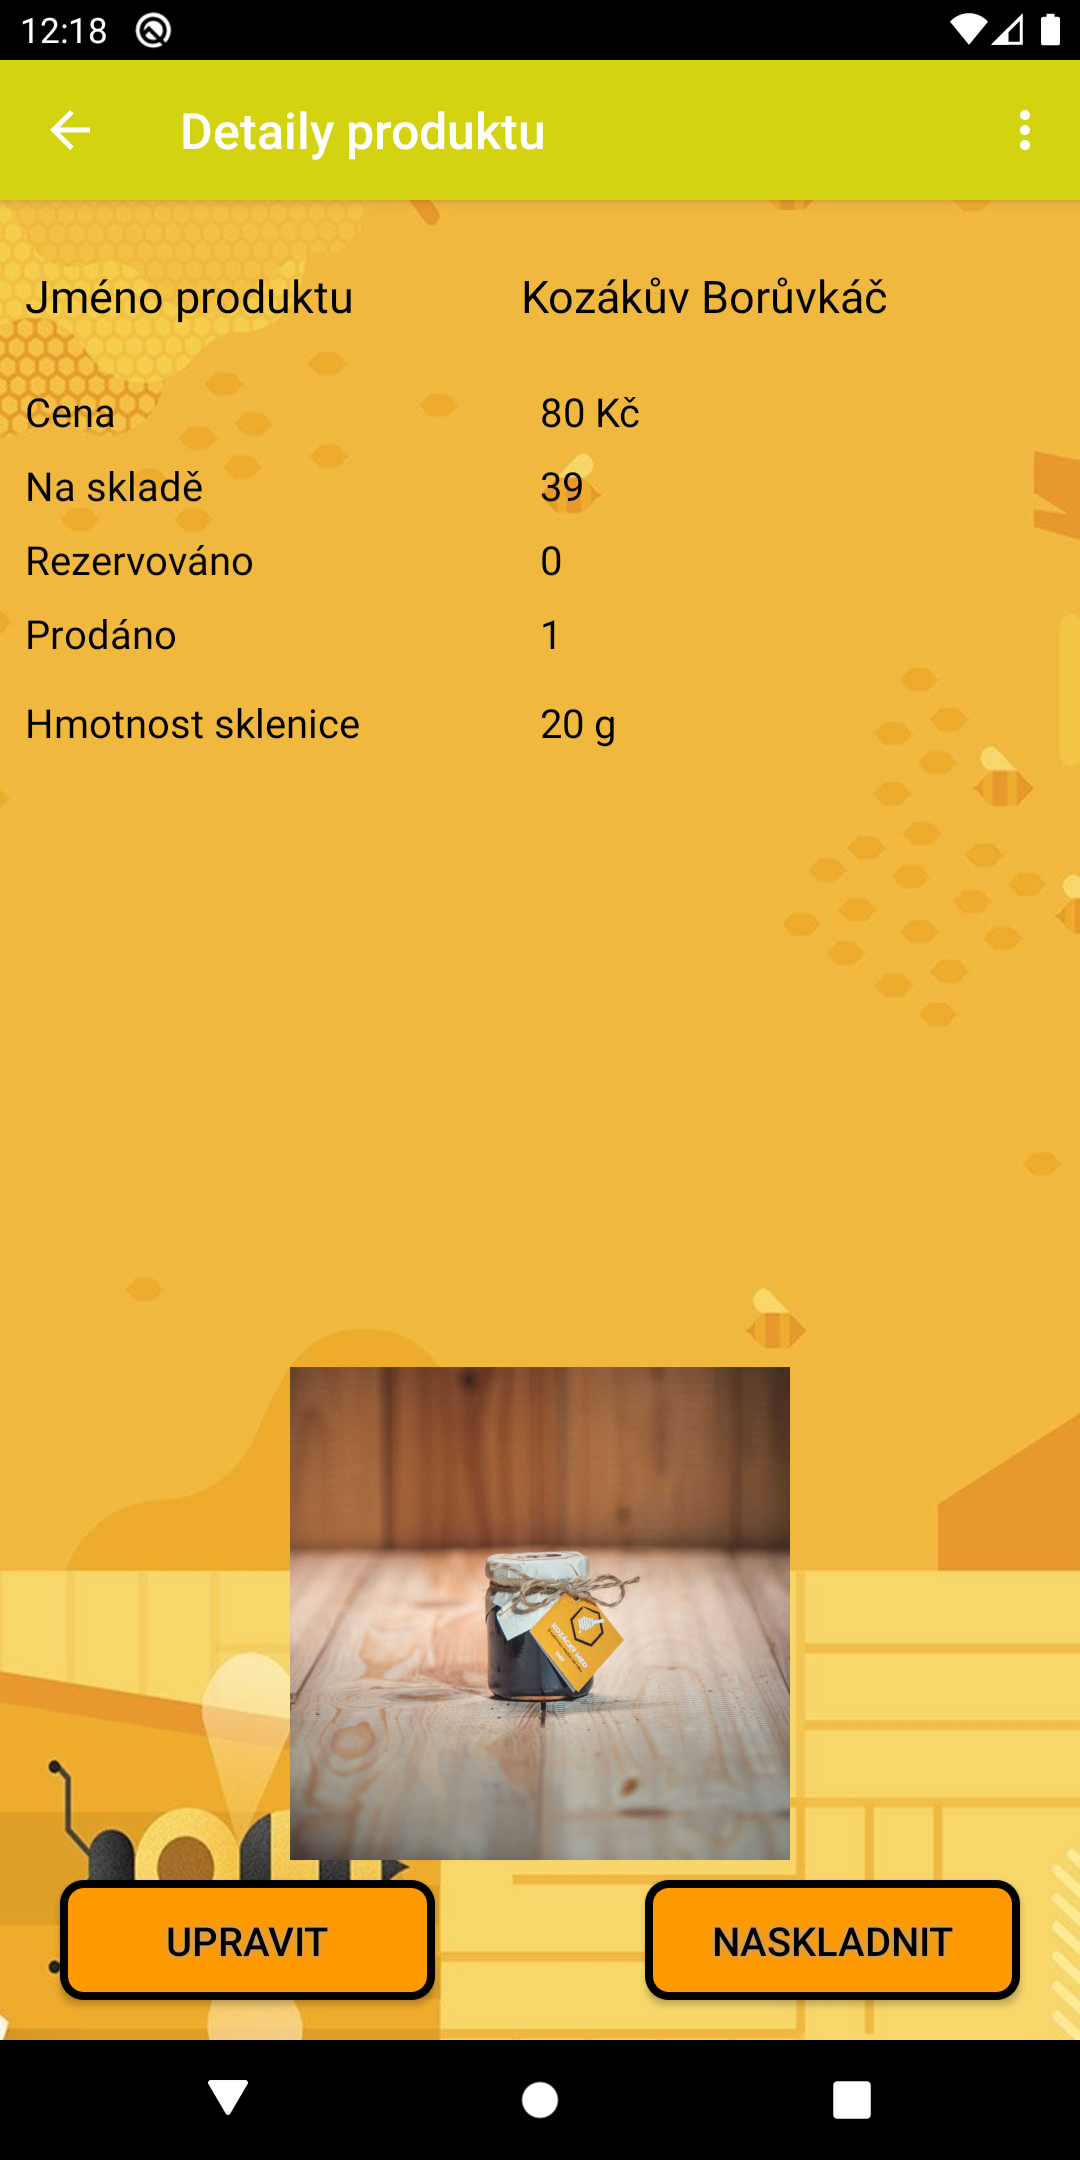
\includegraphics[width=\textwidth]{img/product_detail.png}
	  \caption{Detail produktu}
	  \label{fig:product_det}
	\end{subfigure}
	%
	\caption{Detaily}
	\label{fig:detail_cont}
\end{figure}

Obrazovky sloužící k zobrazení vlastností konkrétního objektu a dodatečnými akcemi na ním.

Na obrázku \ref{fig:order_det} je příklad detailů aktivní objednávky. Kromě informací o objednávce
a seznamu objednaných produktů jsou zde tlačítka pro zrušení objednávky a dokončení objednávky.
Zrušení smaže objednávku z databáze a obnoví rezervované produkty. Dokončení objednávky označí objednávku
jako dokončenou a odebere rezervované produkty, které přičte k prodaným.

Na obrázku \ref{fig:product_det} je detail produktu. Kromě zobrazení jeho vlastností je zde také tlačítko,
kterým lze přidat počet produktu na sklad. Tlačítko pro úpravu otevře produkt ve formuláři, kde je možné měnit
jeho vlastnosti. V pravém horním rohu je menu, které umožní produktu přidat nebo odebrat obrázek (aktivní je pouze
jedna možnost, podle toho, zda produkt již obrázek má či nikoliv).
%
\section{Přidávací formuláře}
\begin{figure}[H]
	\centering
	\begin{subfigure}{.45\textwidth}
	  \centering
	  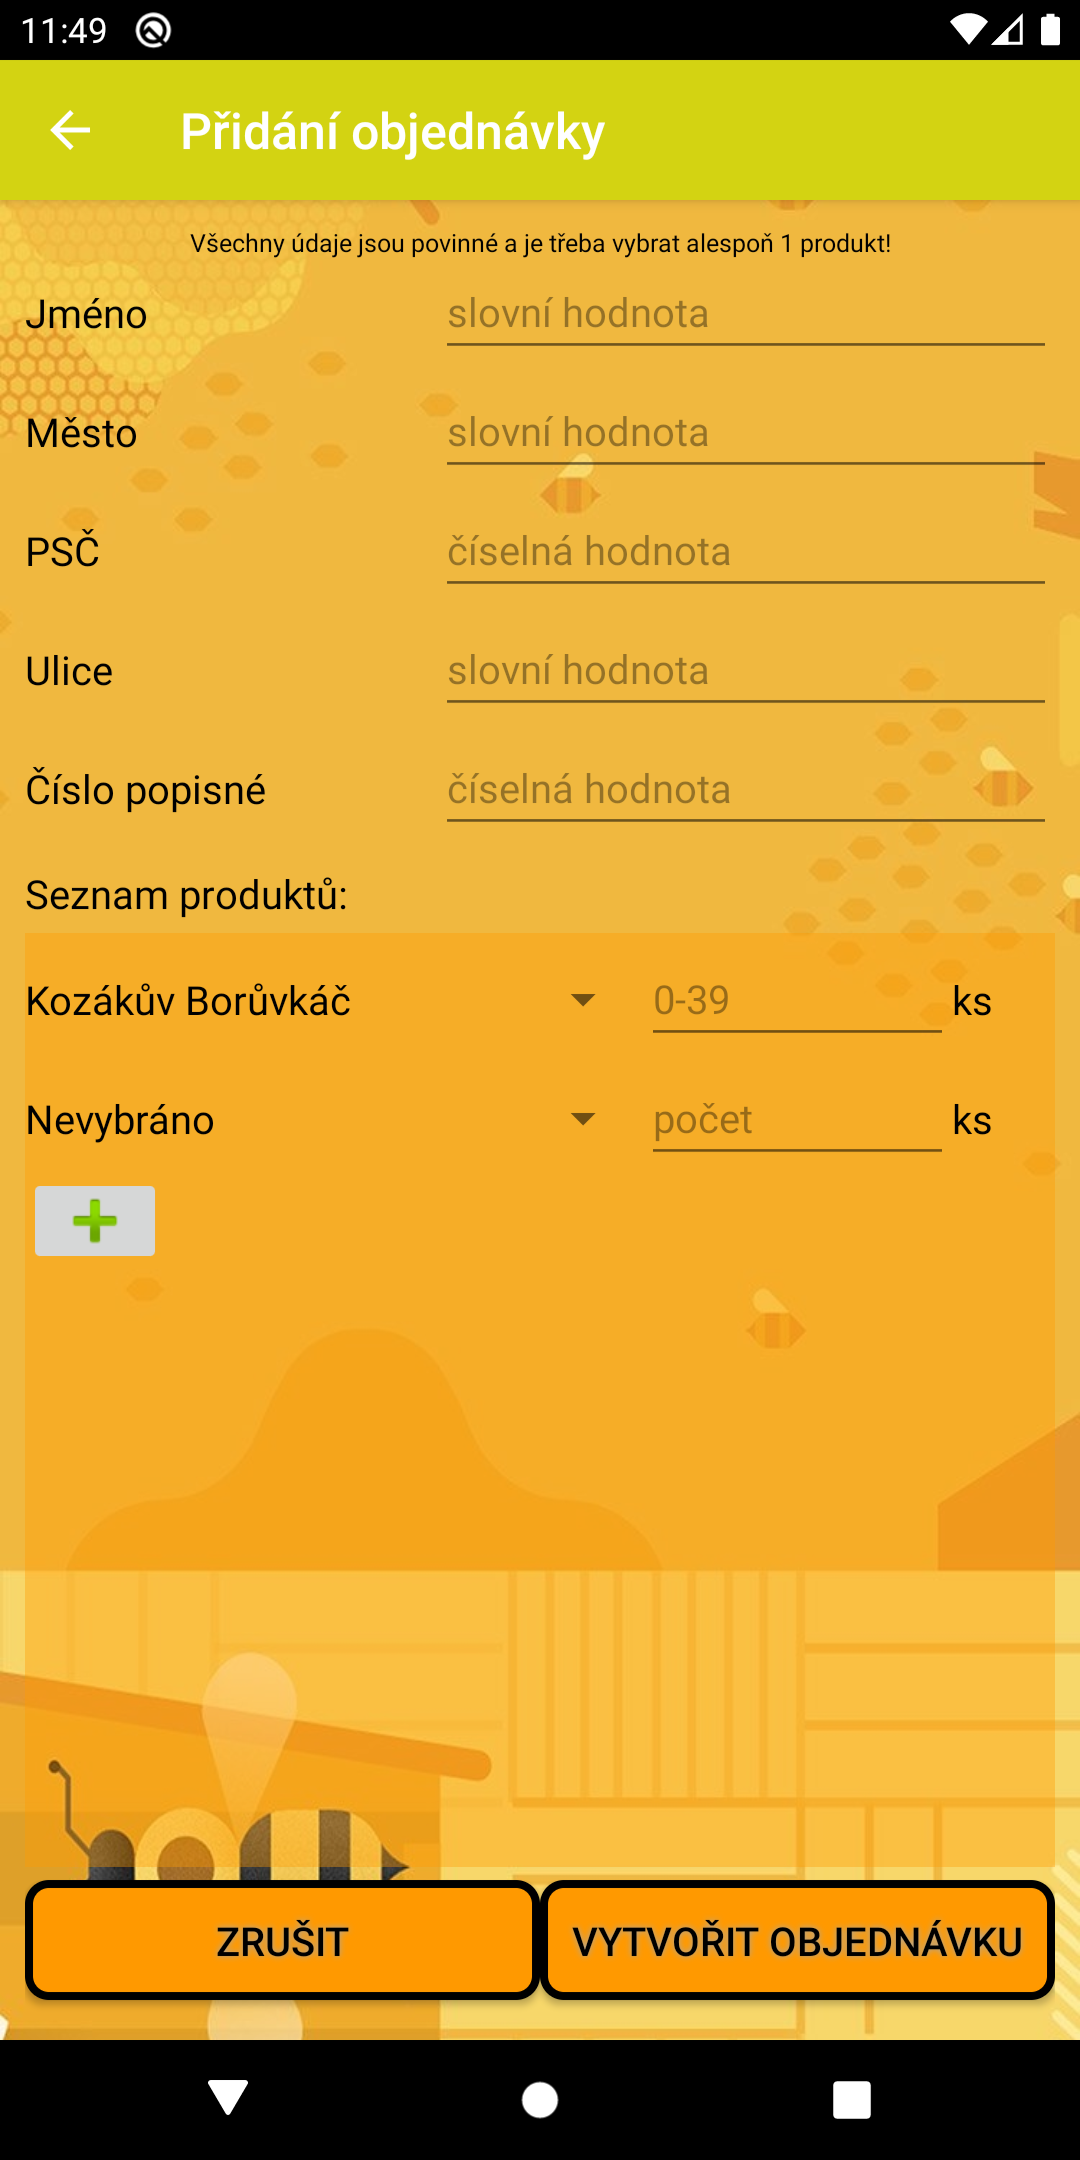
\includegraphics[width=\textwidth]{img/order_creation.png}
	  \caption{Vytvoření nové objednávky}
	  \label{fig:order_add}
	\end{subfigure}
	%
	\begin{subfigure}{.45\textwidth}
	  \centering
	  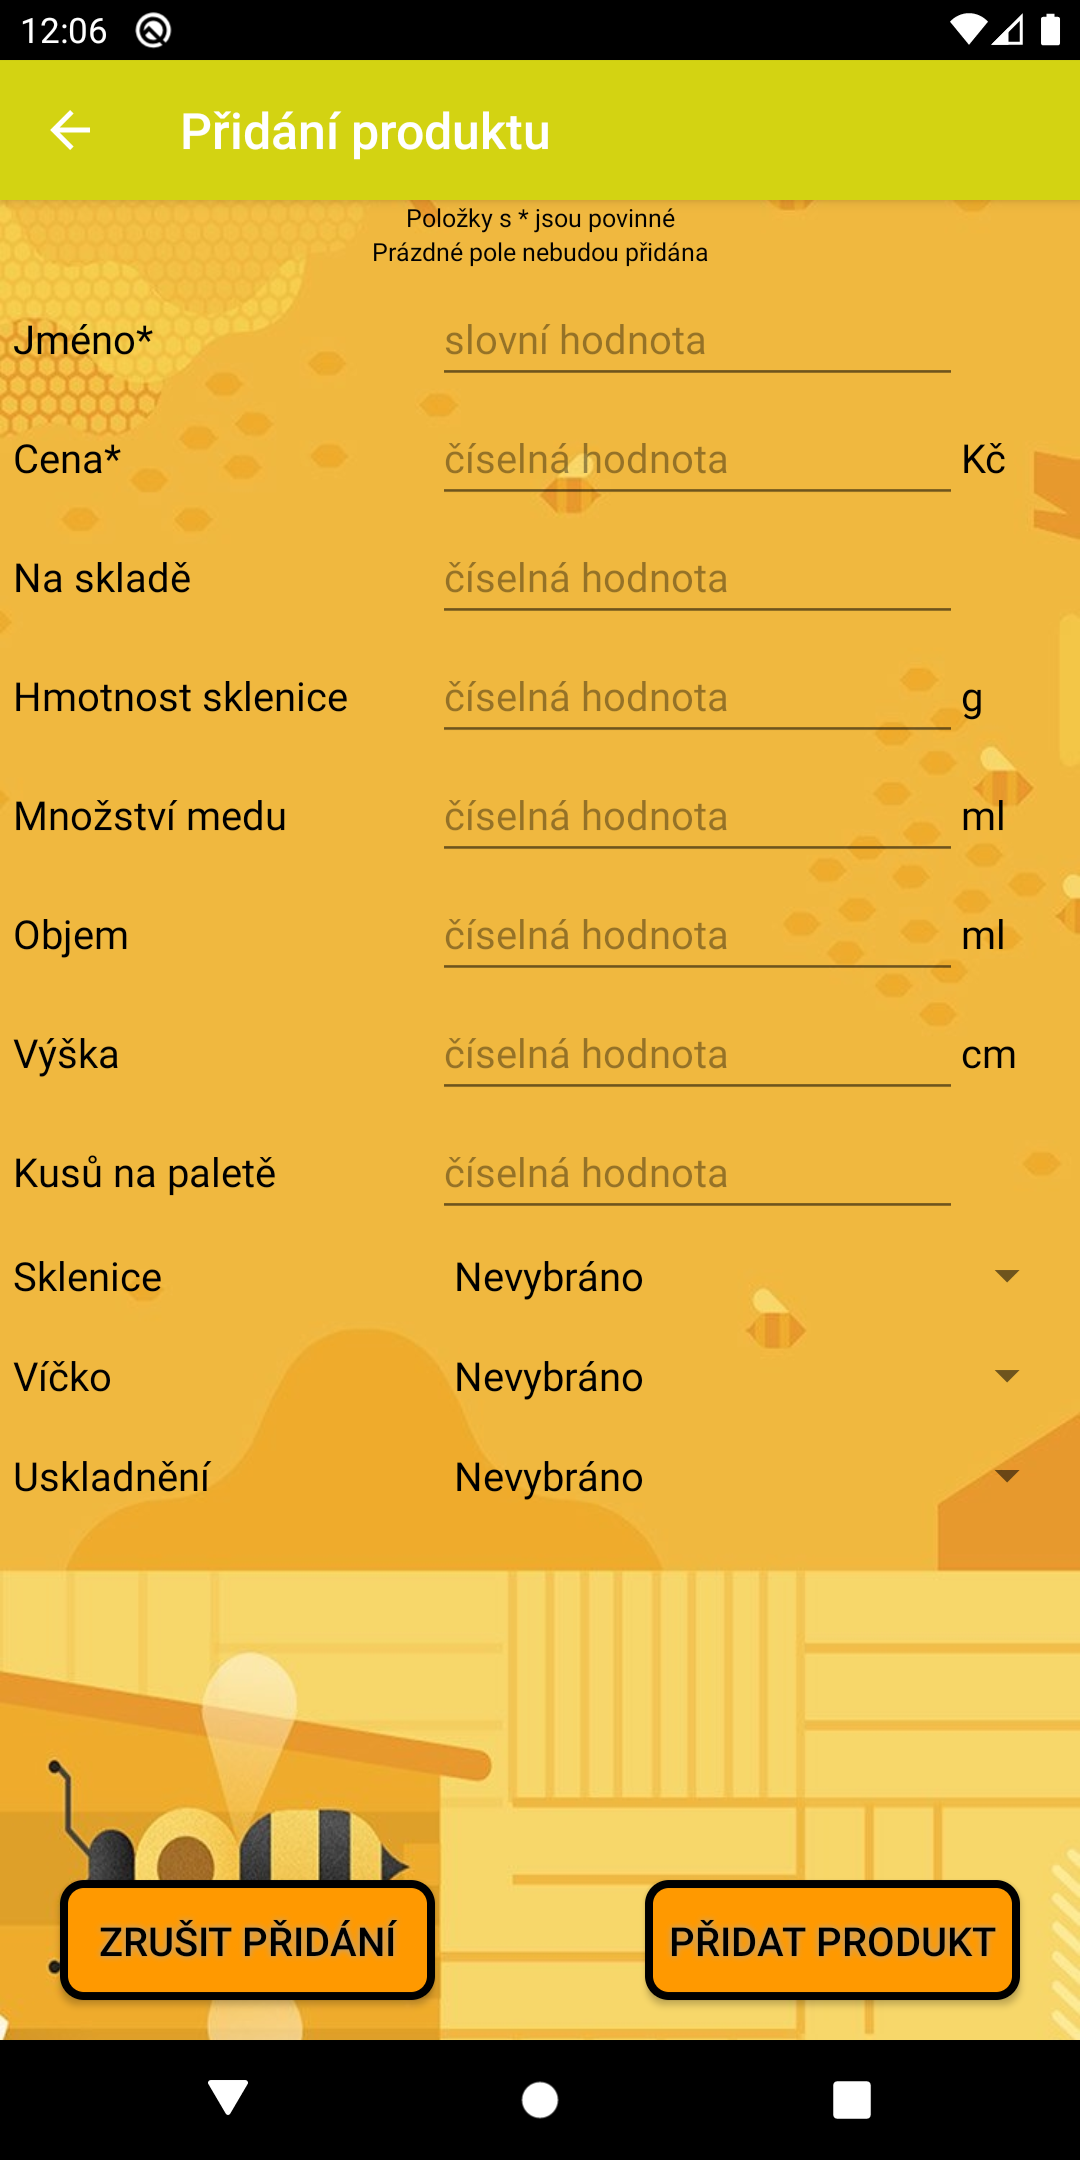
\includegraphics[width=\textwidth]{img/product_addition.png}
	  \caption{Vytvoření nového produktu}
	  \label{fig:product_add}
	\end{subfigure}
	%
	\caption{Přidávací formuláře}
	\label{fig:creation_cont}
\end{figure}

Obrázek \ref{fig:order_add} je aktivita pro přidání objednávky. Jsou zde statická pole, která musí být zadána.
Těmi jsou jméno a adresa. Poté je zde tabulka produktů objednávky. Tabulka je z počátku prázdná a je zde
pouze tlačítko pro přidání nové řádky. Nová řádka má Spinner (dropdown menu), ze kterého se vybere produkt a
vstupní pole pro počet produktů. Další řádku není možné přidat, pokud na předchozí nebyl vybrán nějaký produkt.
Při vyčerpání možností (vybráním všech produktů) je tlačítko přidání odebráno. Řádky je možné odebrat pomocí
kontextového menu (podržením na řádku, kterou si uživatel přeje odebrat).

Obrázek \ref{fig:product_add} je aktivita pro přidání produktu. První tři položky jsou vlastnosti produktu
(jméno, cena, počet na skladě) a proto jsou statické. Zbylé položky jsou přidány podle vlastností získané 
z databáze. Upravení produktu používá velmi podobné rozhraní, kdy jediným rozdílem je, že úprava nemá vstup
s počtem na skladě.
%
\section{Dialogy a chyby}
\begin{figure}[H]
	\centering
	\begin{subfigure}{.45\textwidth}
	  \centering
	  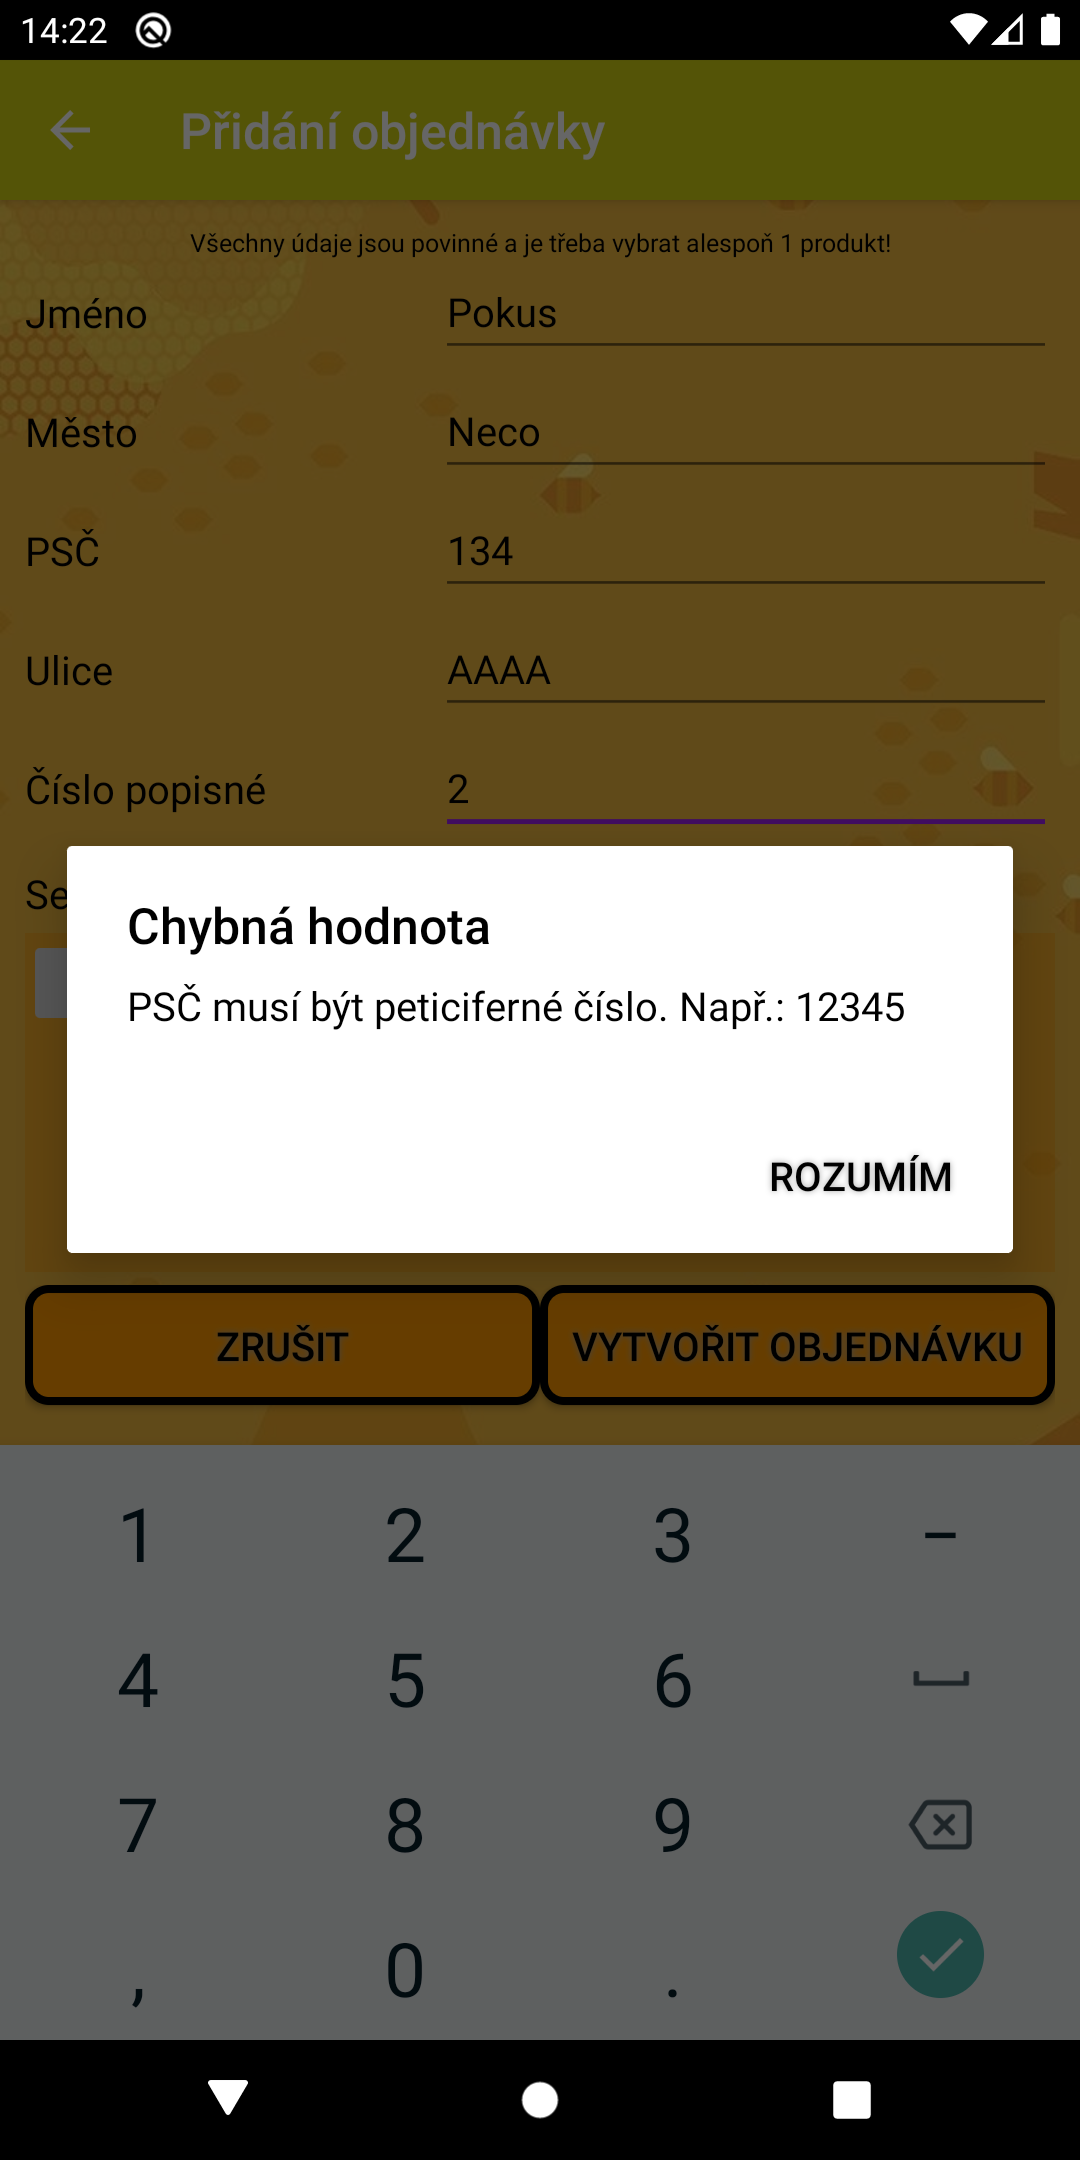
\includegraphics[width=.9\textwidth]{img/error_dialog.png}
	  \caption{Příklad dialogu chyby}
	  \label{fig:dialog_error}
	\end{subfigure}
	%
	\begin{subfigure}{.45\textwidth}
	  \centering
	  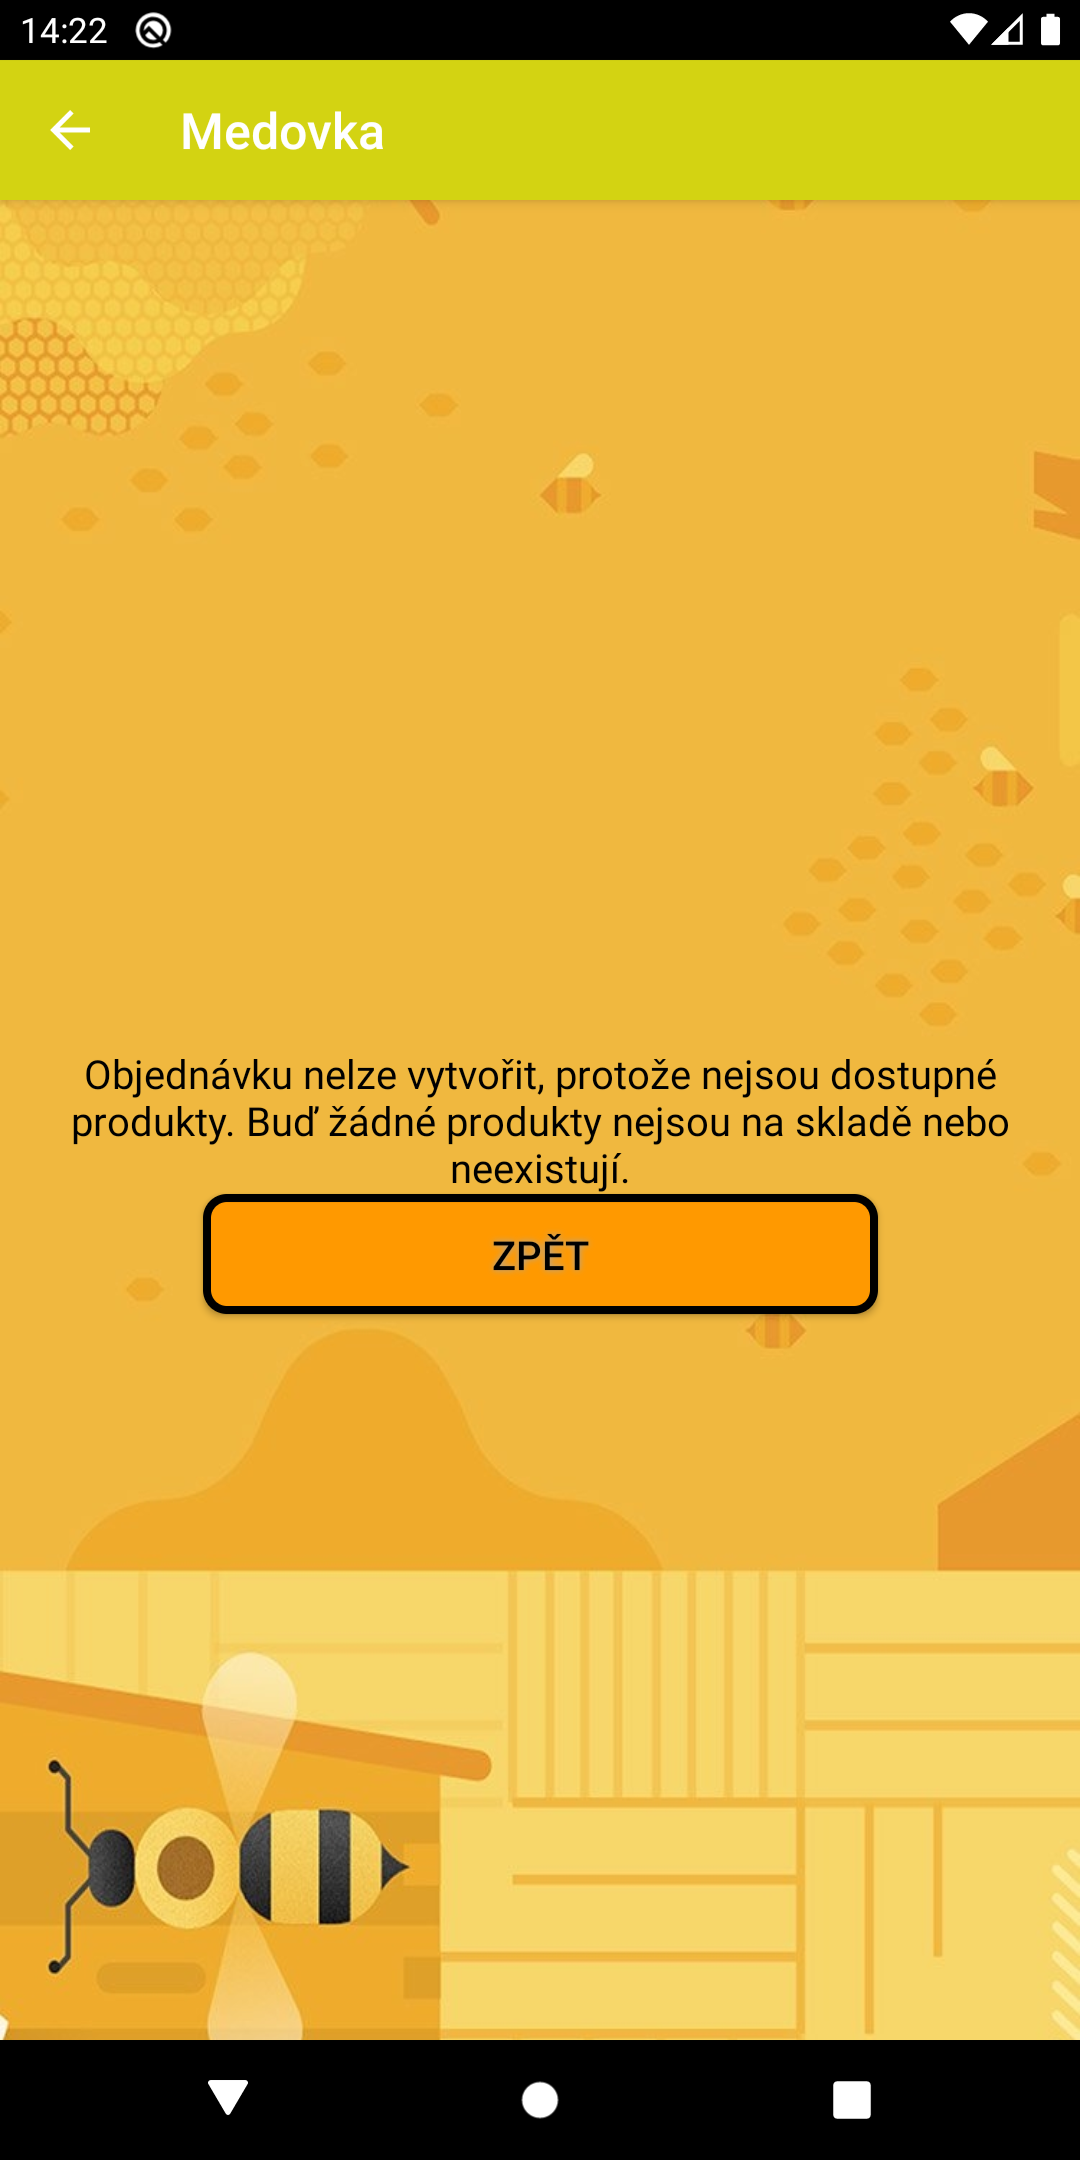
\includegraphics[width=.9\textwidth]{img/error_label.png}
	  \caption{Příklad chyby popiskem}
	  \label{fig:label_error}
	\end{subfigure}
	%
	\caption{Příklady chyb}
	\label{fig:error_cont}
\end{figure}
%
Pro informování uživatele o chybě je použit buď dialog (např. obrázek \ref{fig:dialog_error} 
nebo popisek (např. obrázek \ref{fig:label_error}).

Dialogy navíc slouží k interakci s uživatelem, kdy se uživatele ptají, zda-li chce provést zvolenou akci
nebo ji zrušit. V případě naskladnění produktů je použit dialog se vstupem a počet produktů, které mají
být doplněny je zadán v tomto dialogu.
%
\chapter{Testy a reakce}
%
\section{Test 1}
Tento test byl proveden, když aplikace stále měla hodně bugů. O některých jsem již věděl. 
Hlavním cílem tohoto testování bylo zjistit zda-li si tester myslí, že návrh rozhraní je přijatelný.
\subsection{Testerova zpráva}
\begin{itemize}
	\item doplnění produktu - vyskočit klávesnice
	\item edit/nový produkt - zadání ceny
	\item při kopírování nového produktu otevřít rovnou editaci
	\item odebírání produktu - při kliknutí na check box se nezobrazí tlačítko pro odstranění produktu
	\item po přidání objednávky zobrazit informaci o přidání objednávky
	\item při odstranění řádky při přidávání objednávky se přidá další tlačítko pro přidání produktu
	\item při objednání více produktů upozornit na nulové množství
	\item přidat jednotky pro produkty
\end{itemize}
%
\subsection{Reakce}
Protože jsem s testerem volal během testování, tak tester neudělal bod úplně ke všemu co zmínil. K návrhu 
tester říkal, že většina věcí by se těžko dala udělat líp. Ovšem jednou z velkých změn, kterou mi
doporučil bylo, aby se po zkopírování otevřel zkopírovaný produkt k editaci. Dříve jsem pouze 
produkt zkopíroval a informoval uživatele o úspěchu.

Mimo tuto změnu mi tester našel množství bugů zmíněné ve zprávě. Všechny body, které tester zmínil 
jsem vzal v potaz a opravil, či přepracoval.
%
\section{Test 2}
\subsection{Testerova zpráva}
Testování proběhlo na emulátoru v systému Windows za asistence vývojáře. Vyzkoušel jsem si snad všechny funkce, které aplikace nabízí. GUI se mi z grafického pohledu líbilo.
U vytváření nových objednávek jsme narazili na pár problémů. Při dodržování určitých kroků mohlo dojít k tomu, že šlo mít v objednávce 2x ten samý typ medu, což pak vyvolávalo problémy. Vývojář o tomto problému věděl a říkal, že pracuje na jeho odstranění. Druhá chyba na kterou jsem narazil, nebyla až tak závažná. Jednalo se o to, že u PSČ a č.p. šlo začít číslem 0, které pak byly vymazány. Tyto hodnoty jsou ale nesmyslné a nepředpokládal bych je v reálném využití aplikace.
Jedna věc kterou bych možná změnil, je přístup u editace produktů. Líbilo by se mi kdybych mohl odstranit produkt v "přehledu produktů". To samé by šlo i s přidáním produktu, případně jeho kopírování
\subsection{Reakce}
Jak tester zmínil o bugu, kdy při změně produktu ve Spinneru, se občas produkt neodstranil z ostatních 
Spinnerů jsem věděl. Na tomto problému jsem strávil poměrně dlouho dobu, než jsem nakonec způsob,
jakým jsou produkty ve Spinnerech aktualizovány, zcela předělal (ačkoliv ne tak elegantně, 
jak jsem se původně pokoušel). Tudíž tato chyba by měla být opravena.

Druhou chybu (0 na začátku čísla) jsem vzal jako chybnou hodnotu a pokud se uživatel pokusí 
zadat PSČ nebo č.p. s 0 na začátku tak je dialogem informován, že číslo nesmí začínat 0. Toto také
zajišťuje, že číslo nikdy nebude 0.

Akce pro kopírování/ odebrání produktu přímo z přehledu jsem také zvažoval. Nakonec jsem se
ale rozhodl udělat pro každou akci vlastní list, protože jsem chtěl, aby bylo možné mazání více
produktů zároveň. Původně jsem chtěl umožnit i kopírování více produktů, ale rozhodl
jsem se proti tomu. Myslím si, že kopírovat či odstranit produkt přímo z přehledu je smysluplná
akce a mohla by být přidána jako rozšíření aplikace, ovšem pro hlavní zamýšlenou funkčnost věřím,
že je mé řešení více než dostačující.
\section{Test 3}
\subsection{Testerova zpráva}
Tato zpráva je přiložena na konci této dokumentace (za závěrem).
\subsection{Reakce}
K první vítce, zarovnání textu, v sekci "O aplikaci" jsem nastavil zarovnání, ovšem mě osobně se
líbilo předchozí zarovnání.

Přidání vlastního políčka (atributu - vlastnosti) u vytváření produktu je funkce, kterou jsem
odřízl za časových důvodů. 
Původně jsem tuto funkci v aplikaci chtěl mít, ale přidat tuto funkci by znamenalo navíc den nebo dva
vývoje a již teď odevzdávám práci s velkým zpožděním.

Možnost kopírování objednávky mě ani nenapadlo kvůli tomu, že ve velkém počtu objednávek by se těžko
hledala jedna konkrétní. S přidáním různých filtrů by to ale nemusel být problém a jednalo by se o
pěknou funkci.

Grafický problém posunutí tlačítka je bohužel způsoben tím, že aplikace není plně škálovatelná mezi
zařízeními. Aplikaci jsem zkoušel na různých displejích a v podstatě je použitelná i na displeji s
3.3" a rozlišením 240x400. Ovšem na menších displejích vzniká prolbém, že tlačítka, do kterých se text
nevejde na jednu řádku, se "roztáhnou" do výšky, protože text se napíše do sloupce. Tomuto je poměrně 
těžké zabránit a u mobilních aplikací se většinou dělají stejné layouty pro různé velikosti displejů,
které mají zbaránit tomuto a podobným problémům.
%
\chapter{Závěr}
Zadání aplikace mi bylo zadáno kamarádem, jako aplikace, kterou by mohl i využívat. Bohužel jsem velmi podcenil
složitost aplikace a strávil jsem mnohem větší množství času implementováním základních funkcí, než
jsem původně odhadoval. Z tohoto důvodu aplikace není moc propracovaná a hodně funkcí jsem byl nucen
ořezat, abych aplikaci stihl odevzdat jako semestrální práci. Na aplikaci je spoustu funkcí, kterými 
by bylo vhodné ji rozšířit. Díky relativně solidnímu základu by nemělo být složité většinu funkcí
implementovat.

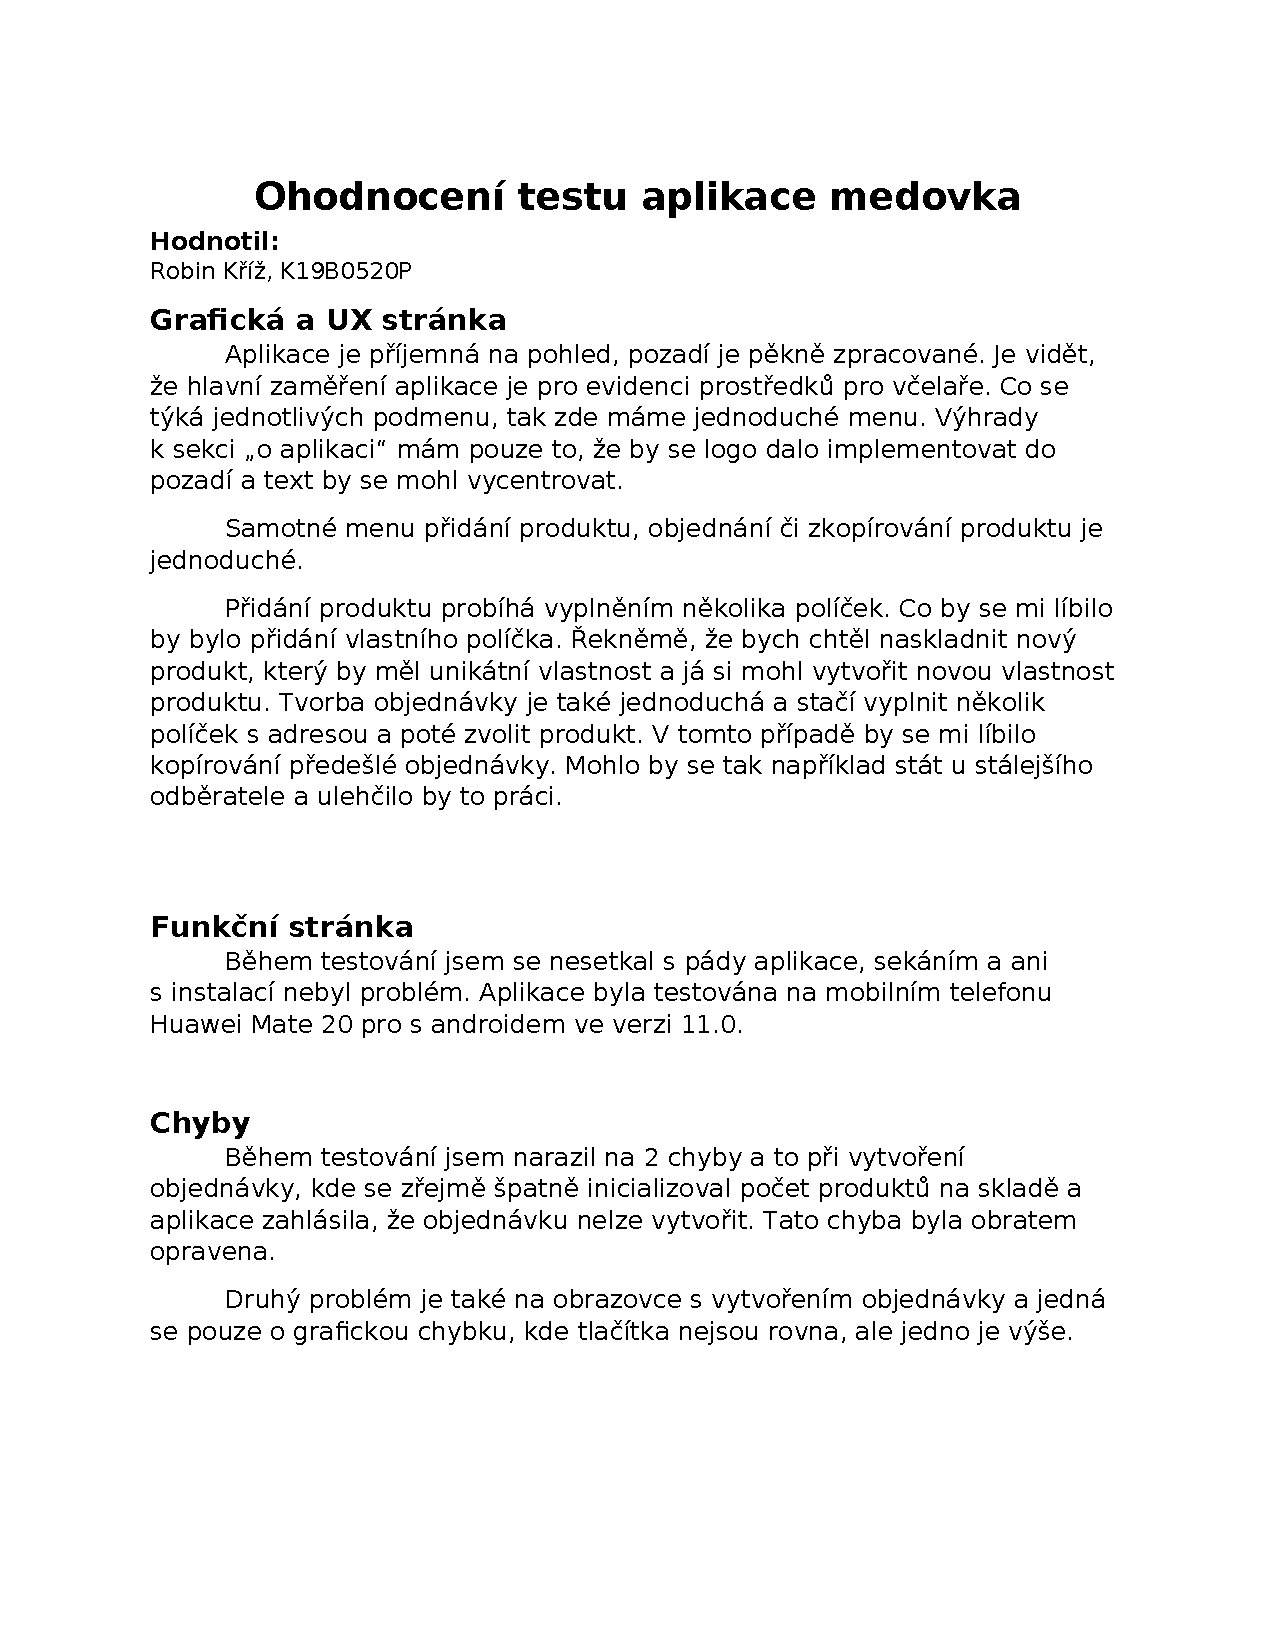
\includepdf[pages=-,width=\textwidth]{./testRobinKriz.pdf}
%
\end{document}
